%\documentclass{article}
%\usepackage{beamerarticle}
\documentclass[serif,ignorenonframetext]{beamer}

% Macros for MATH 110 course dates

\newcommand{\commonTheme}{metropolis}
\newcommand{\commonColorTheme}{metropolis}

\newcommand{\commonAuthor}{Edward Doolittle}
\newcommand{\commonInstitute}{Department of Indigenous Knowledge and
  Science \\ First Nations University of Canada}
\newcommand{\commonCourse}{MATH 110 Calculus I}
\newcommand{\commonTerm}{202510}
\newcommand{\commonDate}{January 6, 2025}

% Review Material

% Lab 0
\newcommand{\commonEventNegativeOne}{LabNegativeOne}
\newcommand{\commonDateLabNegativeOne}{Monday, January 6, 2025}
\newcommand{\commonTitleLabNegativeOne}{MATH 110 Lab 0}
\newcommand{\commonSubtitleLabNegativeOne}{No Lab; Course Opens}

% Section 001
\newcommand{\commonEventZeroZeroOne}{ZeroZeroOne}
\newcommand{\commonDateZeroZeroOne}{Tuesday, January 7, 2025}
\newcommand{\commonTitleZeroZeroOne}{MATH 110 Review 0.1}
\newcommand{\commonSubtitleZeroZeroOne}{Review of Algebra}
\newcommand{\commonPSTitleZeroZeroOne}{MATH 110 Review Problem Set 0.1}

% Section 00A
\newcommand{\commonEventZeroZeroA}{ZeroZeroA}
\newcommand{\commonDateZeroZeroA}{Tuesday, January 7, 2025}
\newcommand{\commonTitleZeroZeroA}{MATH 110 Review 0.A}
\newcommand{\commonSubtitleZeroZeroA}{Review of Inequalities and
  Absolute Values}
\newcommand{\commonPSTitleZeroZeroA}{MATH 110 Review Problem Set 0.A}

% Section 00B
\newcommand{\commonEventZeroZeroB}{ZeroZeroB}
\newcommand{\commonDateZeroZeroB}{Tuesday, January 7, 2025}
\newcommand{\commonTitleZeroZeroB}{MATH 110 Review 0.B}
\newcommand{\commonSubtitleZeroZeroB}{Review of Coordinate Geometry
  and Lines}
\newcommand{\commonPSTitleZeroZeroB}{MATH 110 Review Problem Set 0.B}

% Section 00C
\newcommand{\commonEventZeroZeroC}{ZeroZeroC}
\newcommand{\commonDateZeroZeroC}{Thursday, January 9, 2025}
\newcommand{\commonTitleZeroZeroC}{MATH 110 Review 0.C}
\newcommand{\commonSubtitleZeroZeroC}{Review of Graphs of Second
  Degree Equations}
\newcommand{\commonPSTitleZeroZeroC}{MATH 110 Review Problem Set 0.C}

% Section 00D
\newcommand{\commonEventZeroZeroD}{ZeroZeroD}
\newcommand{\commonDateZeroZeroD}{Thursday, January 9, 2025}
\newcommand{\commonTitleZeroZeroD}{MATH 110 Review 0.D}
\newcommand{\commonSubtitleZeroZeroD}{Review of Trigonometry}
\newcommand{\commonPSTitleZeroZeroD}{MATH 110 Review Problem Set 0.D}

% Section 011
\newcommand{\commonEventZeroOneOne}{ZeroOneOne}
\newcommand{\commonDateZeroOneOne}{Thursday, January 9, 2025}
\newcommand{\commonTitleZeroOneOne}{MATH 110 Review 1.1}
\newcommand{\commonSubtitleZeroOneOne}{Review of Functions}
\newcommand{\commonPSTitleZeroOneOne}{MATH 110 Review Problem Set 1.1}


% Main Course

% Lab 1
\newcommand{\commonEventZero}{LabZero}
\newcommand{\commonDateLabZero}{Monday, January 13, 2025}
\newcommand{\commonTitleLabZero}{MATH 110 Lab 1}
\newcommand{\commonSubtitleLabZero}{Quiz 0: STACK, Onboarding}

% Section 1.4
\newcommand{\commonEventOne}{ZeroOneFour}
\newcommand{\commonDateZeroOneFour}{Tuesday, January 14, 2025}
\newcommand{\commonTitleZeroOneFour}{MATH 110 Lecture 1.4}
\newcommand{\commonSubtitleZeroOneFour}{The Tangent and Velocity Problems}
\newcommand{\commonPSTitleZeroOneFour}{MATH 110 Problem Set 1.4}

% Section 1.5
\newcommand{\commonEventTwo}{ZeroOneFive}
\newcommand{\commonDateZeroOneFive}{Thursday, January 16, 2025}
\newcommand{\commonTitleZeroOneFive}{MATH 110 Lecture 1.5}
\newcommand{\commonSubtitleZeroOneFive}{The Limit of a Function}
\newcommand{\commonPSTitleZeroOneFive}{MATH 110 Problem Set 1.5}

% Lab 2
\newcommand{\commonEventThree}{LabOne}
\newcommand{\commonDateLabOne}{Monday, January 20, 2025}
\newcommand{\commonTitleLabOne}{MATH 110 Lab 2}
\newcommand{\commonSubtitleLabOne}{Quiz 1: Review}

% Section 1.6
\newcommand{\commonEventFour}{ZeroOneSix}
\newcommand{\commonDateZeroOneSix}{Tuesday, January 21, 2025}
\newcommand{\commonTitleZeroOneSix}{MATH 110 Lecture 1.6}
\newcommand{\commonSubtitleZeroOneSix}{Calculating Limits Using the Limit Laws}
\newcommand{\commonPSTitleZeroOneSix}{MATH 110 Problem Set 1.6}

% Section 1.7
\newcommand{\commonEventFive}{ZeroOneSeven}
\newcommand{\commonDateZeroOneSeven}{(Not covered)}
\newcommand{\commonTitleZeroOneSeven}{MATH 110 Lecture 1.7}
\newcommand{\commonSubtitleZeroOneSeven}{The Precise Definition of a Limit}
\newcommand{\commonPSTitleZeroOneSeven}{MATH 110 Problem Set 1.7}

% Section 1.8
\newcommand{\commonEventSix}{ZeroOneEight}
\newcommand{\commonDateZeroOneEight}{Thursday, January 23, 2025}
\newcommand{\commonTitleZeroOneEight}{MATH 110 Lecture 1.8}
\newcommand{\commonSubtitleZeroOneEight}{Continuity}
\newcommand{\commonPSTitleZeroOneEight}{MATH 110 Problem Set 1.8}

% Lab 3
\newcommand{\commonEventSeven}{LabTwo}
\newcommand{\commonDateLabTwo}{Monday, January 27, 2025}
\newcommand{\commonTitleLabTwo}{MATH 110 Lab 3}
\newcommand{\commonSubtitleLabTwo}{Quiz 2: Sections 1.4, 1.5}

% Section 2.1
\newcommand{\commonEventEight}{ZeroTwoOne}
\newcommand{\commonDateZeroTwoOne}{Tuesday, January 28, 2025}
\newcommand{\commonTitleZeroTwoOne}{MATH 110 Lecture 2.1}
\newcommand{\commonSubtitleZeroTwoOne}{Derivatives and Rates of Change}
\newcommand{\commonPSTitleZeroTwoOne}{MATH 110 Problem Set 2.1}

% Section 2.2
\newcommand{\commonEventNine}{ZeroTwoTwo}
\newcommand{\commonDateZeroTwoTwo}{Thursday, January 30, 2025}
\newcommand{\commonTitleZeroTwoTwo}{MATH 110 Lecture 2.2}
\newcommand{\commonSubtitleZeroTwoTwo}{The Derivative as a Function}
\newcommand{\commonPSTitleZeroTwoTwo}{MATH 110 Problem Set 2.2}

% Lab 4
\newcommand{\commonEventTen}{LabThree}
\newcommand{\commonDateMTOne}{Monday, February 3, 2025} 
\newcommand{\commonDateLabThree}{Monday, February 3, 2025}
\newcommand{\commonTitleLabThree}{MATH 110 Lab 4}
\newcommand{\commonSubtitleLabThree}{Midterm: Review, Chapter 1}

% Section 2.3
\newcommand{\commonEventEleven}{ZeroTwoThree}
\newcommand{\commonDateZeroTwoThree}{Tuesday, February 4, 2025}
\newcommand{\commonTitleZeroTwoThree}{MATH 110 Lecture 2.3}
\newcommand{\commonSubtitleZeroTwoThree}{Differentiation Formulas}
\newcommand{\commonPSTitleZeroTwoThree}{MATH 110 Problem Set 2.3}

% Section 2.4
\newcommand{\commonEventTwelve}{ZeroTwoFour}
\newcommand{\commonDateZeroTwoFour}{Thursday, February 6, 2025}
\newcommand{\commonTitleZeroTwoFour}{MATH 110 Lecture 2.4}
\newcommand{\commonSubtitleZeroTwoFour}{Derivatives of Trigonometric Functions}
\newcommand{\commonPSTitleZeroTwoFour}{MATH 110 Problem Set 2.4}

% Lab 5
\newcommand{\commonEventThirteen}{LabFour}
\newcommand{\commonDateLabFour}{Monday, February 10, 2025}
\newcommand{\commonTitleLabFour}{MATH 110 Lab 5}
\newcommand{\commonSubtitleLabFour}{Quiz 3: Sections 2.1, 2.2}

% Section 2.5
\newcommand{\commonEventFourteen}{ZeroTwoFive}
\newcommand{\commonDateZeroTwoFive}{Tuesday, February 11, 2025}
\newcommand{\commonTitleZeroTwoFive}{MATH 110 Lecture 2.5}
\newcommand{\commonSubtitleZeroTwoFive}{The Chain Rule}
\newcommand{\commonPSTitleZeroTwoFive}{MATH 110 Problem Set 2.5}

% Section 2.6
\newcommand{\commonEventFifteen}{ZeroTwoSix}
\newcommand{\commonDateZeroTwoSix}{Thursday, February 13, 2025}
\newcommand{\commonTitleZeroTwoSix}{MATH 110 Lecture 2.6}
\newcommand{\commonSubtitleZeroTwoSix}{Implicit Differentiation}
\newcommand{\commonPSTitleZeroTwoSix}{MATH 110 Problem Set 2.6}

% Lab 6
\newcommand{\commonEventSixteen}{LabFive}
\newcommand{\commonDateLabFive}{Monday, February 24, 2025}
\newcommand{\commonTitleLabFive}{MATH 110 Lab 6}
\newcommand{\commonSubtitleLabFive}{Quiz 4: Sections 2.3, 2.4}

% Section 2.7
\newcommand{\commonEventSeventeen}{ZeroTwoSeven}
\newcommand{\commonDateZeroTwoSeven}{Tuesday, February 25, 2025}
\newcommand{\commonTitleZeroTwoSeven}{MATH 110 Lecture 2.7}
\newcommand{\commonSubtitleZeroTwoSeven}{Rates of Change in the
  Natural and Social Sciences}
\newcommand{\commonPSTitleZeroTwoSeven}{MATH 110 Problem Set 2.7}

% Section 2.8
\newcommand{\commonEventEighteen}{ZeroTwoEight}
\newcommand{\commonDateZeroTwoEight}{Thursday, February 27, 2025}
\newcommand{\commonTitleZeroTwoEight}{MATH 110 Lecture 2.8}
\newcommand{\commonSubtitleZeroTwoEight}{Related Rates}
\newcommand{\commonPSTitleZeroTwoEight}{MATH 110 Problem Set 2.8}

% Lab 7
\newcommand{\commonEventNineteen}{LabSix}
\newcommand{\commonDateLabSix}{Monday, March 3, 2025}
\newcommand{\commonTitleLabSix}{MATH 110 Lab 7}
\newcommand{\commonSubtitleLabSix}{Quiz 5: Sections 2.5, 2.6}

% Section 3.1
\newcommand{\commonEventTwenty}{ZeroThreeOne}
\newcommand{\commonDateZeroThreeOne}{Tuesday, March 4, 2025}
\newcommand{\commonTitleZeroThreeOne}{MATH 110 Lecture 3.1}
\newcommand{\commonSubtitleZeroThreeOne}{Maximum and Minimum Values}
\newcommand{\commonPSTitleZeroThreeOne}{MATH 11 Problem Set 3.1}

% Section 3.2
\newcommand{\commonEventTwentyOne}{ZeroThreeTwo}
\newcommand{\commonDateZeroThreeTwo}{Thursday, March 6, 2025}
\newcommand{\commonTitleZeroThreeTwo}{MATH 110 Lecture 3.2}
\newcommand{\commonSubtitleZeroThreeTwo}{The Mean Value Theorem}
\newcommand{\commonPSTitleZeroThreeTwo}{MATH 110 Problem Set 3.2}

% Lab 8
\newcommand{\commonEventTwentyTwo}{LabSeven}
\newcommand{\commonDateMTTwo}{Monday, March 10, 2025}
\newcommand{\commonDateLabSeven}{Monday, March 10, 2025}
\newcommand{\commonTitleLabSeven}{MATH 110 Lab 8}
\newcommand{\commonSubtitleLabSeven}{Midterm: Chapter 2}

% Section 3.3
\newcommand{\commonEventTwentyThree}{ZeroThreeThree}
\newcommand{\commonDateZeroThreeThree}{Tuesday, March 11, 2025}
\newcommand{\commonTitleZeroThreeThree}{MATH 110 Lecture 3.3}
\newcommand{\commonSubtitleZeroThreeThree}{How Derivatives Affect the
  Shape of a Graph}
\newcommand{\commonPSTitleZeroThreeThree}{MATH 110 Problem Set 3.3}

% Section 3.4
\newcommand{\commonEventTwentyFour}{ZeroThreeFour}
\newcommand{\commonDateZeroThreeFour}{Thursday, March 13, 2025}
\newcommand{\commonTitleZeroThreeFour}{MATH 110 Lecture 3.4}
\newcommand{\commonSubtitleZeroThreeFour}{Limits at Infinity;
  Horizontal Asymptotes}
\newcommand{\commonPSTitleZeroThreeFour}{MATH 110 Problem Set 3.4}

% Lab 9
\newcommand{\commonEventTwentyFive}{LabEight}
\newcommand{\commonDateLabEight}{Monday, March 17, 2025}
\newcommand{\commonTitleLabEight}{MATH 110 Lab 9}
\newcommand{\commonSubtitleLabEight}{Quiz 6: Sections 3.1, 3.2}

% Section 3.5
\newcommand{\commonEventTwentySix}{ZeroThreeFive}
\newcommand{\commonDateZeroThreeFive}{Tuesday, March 18, 2025}
\newcommand{\commonTitleZeroThreeFive}{MATH 110 Lecture 3.5}
\newcommand{\commonSubtitleZeroThreeFive}{Summary of Curve Sketching}
\newcommand{\commonPSTitleZeroThreeFive}{MATH 110 Problem Set 3.5}

% Section 3.7
\newcommand{\commonEventTwentySeven}{ZeroThreeSeven}
\newcommand{\commonDateZeroThreeSeven}{Thursday, March 20, 2025}
\newcommand{\commonTitleZeroThreeSeven}{MATH 110 Lecture 3.7}
\newcommand{\commonSubtitleZeroThreeSeven}{Optimization Problems}
\newcommand{\commonPSTitleZeroThreeSeven}{MATH 110 Problem Set 3.7}

% Lab 10
\newcommand{\commonEventTwentyEight}{LabNine}
\newcommand{\commonDateLabNine}{Monday, March 24, 2025}
\newcommand{\commonTitleLabNine}{MATH 110 Lab 10}
\newcommand{\commonSubtitleLabNine}{Quiz 7: Sections 3.3, 3.4}

% Section 4.1
\newcommand{\commonEventTwentyNine}{ZeroFourOne}
\newcommand{\commonDateZeroFourOne}{Tuesday, March 25, 2025}
\newcommand{\commonTitleZeroFourOne}{MATH 110 Lecture 4.1}
\newcommand{\commonSubtitleZeroFourOne}{Areas and Distances}
\newcommand{\commonPSTitleZeroFourOne}{MATH 110 Problem Set 4.1}

% Section 4.2
\newcommand{\commonEventThirty}{ZeroFourTwo}
\newcommand{\commonDateZeroFourTwo}{Thursday, March 27, 2025}
\newcommand{\commonTitleZeroFourTwo}{MATH 110 Lecture 4.2}
\newcommand{\commonSubtitleZeroFourTwo}{The Definite Integral}
\newcommand{\commonPSTitleZeroFourTwo}{MATH 110 Problem Set 4.2}

% Lab 11
\newcommand{\commonEventThirtyOne}{LabTen}
\newcommand{\commonDateLabTen}{Monday, March 31, 2025}
\newcommand{\commonTitleLabTen}{MATH 110 Lab 11}
\newcommand{\commonSubtitleLabTen}{Quiz 8: Sections 3.5, 3.7}

% Section 4.3
\newcommand{\commonEventThirtyTwo}{ZeroFourThree}
\newcommand{\commonDateZeroFourThree}{Tuesday, April 1, 2025}
\newcommand{\commonTitleZeroFourThree}{MATH 110 Lecture 4.3}
\newcommand{\commonSubtitleZeroFourThree}{The Fundamental Theorem of Calculus}
\newcommand{\commonPSTitleZeroFourThree}{MATH 110 Problem Set 4.3}

% Section 4.4
\newcommand{\commonEventThirtyThree}{ZeroFourFour}
\newcommand{\commonDateZeroFourFour}{Thursday, April 3, 2025}
\newcommand{\commonTitleZeroFourFour}{MATH 110 Lecture 4.4}
\newcommand{\commonSubtitleZeroFourFour}{Indefinite Integrals and the
  Net Change Theorem}
\newcommand{\commonPSTitleZeroFourFour}{MATH 110 Problem Set 4.4}

% Lab 12
\newcommand{\commonEventThirtyFour}{LabEleven}
\newcommand{\commonDateLabEleven}{Monday, April 7, 2025}
\newcommand{\commonTitleLabEleven}{MATH 110 Lab 12}
\newcommand{\commonSubtitleLabEleven}{Quiz 9: Sections 4.1, 4.2}

% Section 4.5
\newcommand{\commonEventThirtyFive}{ZeroFourFive}
\newcommand{\commonDateZeroFourFive}{Tuesday, April 8, 2025}
\newcommand{\commonTitleZeroFourFive}{MATH 110 Lecture 4.5}
\newcommand{\commonSubtitleZeroFourFive}{The Substitution Rule}
\newcommand{\commonPSTitleZeroFourFive}{MATH 110 Problem Set 4.5}

% Section 5.1
\newcommand{\commonEventThirtySix}{ZeroFiveOne}
\newcommand{\commonDateZeroFiveOne}{Thursday, April 10, 2025}
\newcommand{\commonTitleZeroFiveOne}{MATH 110 Lecture 5.1}
\newcommand{\commonSubtitleZeroFiveOne}{Areas Between Curves}
\newcommand{\commonPSTitleZeroFiveOne}{MATH 110 Problem Set 5.1}

% Lab 13
\newcommand{\commonEventThirtySeven}{LabTwelve}
\newcommand{\commonDateLabTwelve}{Monday, April 14, 2025}
\newcommand{\commonTitleLabTwelve}{MATH 110 Review Lab}
\newcommand{\commonSubtitleLabTwelve}{Bonus Quiz 10: Sections 4.3, 4.4}

% Final Class
\newcommand{\commonEventThirtyEight}{FinalClass}
\newcommand{\commonDateFinalClass}{Tuesday, April 15, 2025}
\newcommand{\commonTitleFinalClass}{MATH 110 Review Class}
\newcommand{\commonSubtitleFinalClass}{Answer Questions, Review for Exam}

% Final Exam
\newcommand{\commonEventThirtyNine}{Final}
\newcommand{\commonDateFinal}{Thursday, April 22, 2025}
\newcommand{\commonTitleFinal}{MATH 110 Final Exam}
\newcommand{\commonSubtitleFinal}{Comprehensive Exam: All Sections}

% Orphaned -- no longer part of the course

% Section 2.9
\newcommand{\commonDateZeroTwoNine}{Not part of the course}
\newcommand{\commonTitleZeroTwoNine}{MATH 110 Lecture 2.9}
\newcommand{\commonSubtitleZeroTwoNine}{Linear Approximations and Differentials}
\newcommand{\commonPSTitleZeroTwoNine}{MATH 110 Problem Set 2.9}


% % Introduction
% \newcommand{\commonEventOneDate}{Wednesday, September 8, 2010}
% \newcommand{\commonEventOneDesc}{Introduction to the Course}
% \newcommand{\commonDateZeroZeroZero}{September 8, 2010}
% \newcommand{\commonTitleZeroZeroZero}{MATH 104 Introduction}
% \newcommand{\commonSubtitleZeroZeroZero}{Outline of the Course}

% % Lecture 1
% \newcommand{\commonEventTwoDate}{Friday, September 10, 2010}
% \newcommand{\commonEventTwoDesc}{Lecture 1: Algebra}
% \newcommand{\commonDateZeroZeroOne}{September 10, 2010}
% \newcommand{\commonTitleZeroZeroOne}{MATH 104 Lecture 1}
% \newcommand{\commonSubtitleZeroZeroOne}{Review of Algebra}
% % associated evaluation ... factor this out?
% \newcommand{\commonPSTitleZeroZeroOne}{MATH 104 Problem Set 1}
% \newcommand{\commonEvalZeroZeroOne}{Quiz 1}
% \newcommand{\commonEvalDateZeroZeroOne}{Wednesday, September 15, 2010}

% % Lecture 2
% \newcommand{\commonEventThreeDate}{Monday, September 13, 2010}
% \newcommand{\commonEventThreeDesc}{Lecture 2: Appendix A}
% \newcommand{\commonDateZeroZeroA}{September 13, 2010}
% \newcommand{\commonTitleZeroZeroA}{MATH 104 Lecture 2}
% \newcommand{\commonSubtitleZeroZeroA}{Appendix A: Numbers, Inequalities, 
%   and Absolute Values}
% % associated evaluation ... factor this out?
% \newcommand{\commonPSTitleZeroZeroA}{MATH 104 Problem Set 2}
% \newcommand{\commonEvalZeroZeroA}{Quiz 2}
% \newcommand{\commonEvalDateZeroZeroA}{Wednesday, September 22, 2010}

% % Review 1
% \newcommand{\commonEventFourDate}{Wednesday, September 15, 2010}
% \newcommand{\commonEventFourDesc}{Review 1: Review Algebra; Quiz 1; Review Appendix A}
% \newcommand{\commonDateRZeroOne}{September 15, 2010}
% \newcommand{\commonTitleRZeroOne}{MATH 104 Review 1}
% \newcommand{\commonSubtitleRZeroOne}{Review of Algebra, Appendix A}

% % Lecture 3
% \newcommand{\commonEventFiveDate}{Friday, September 17, 2010}
% \newcommand{\commonEventFiveDesc}{Lecture 3: Appendix B}
% \newcommand{\commonDateZeroZeroB}{September 17, 2010}
% \newcommand{\commonTitleZeroZeroB}{MATH 104 Lecture 3}
% \newcommand{\commonSubtitleZeroZeroB}{Appendix B: Coordinate Geometry and Lines}
% % associated evaluation ... factor this out?
% \newcommand{\commonPSTitleZeroZeroB}{MATH 104 Problem Set 3}
% \newcommand{\commonEvalZeroZeroB}{Quiz 2}
% \newcommand{\commonEvalDateZeroZeroB}{Wednesday, September 22, 2010}

% % Lecture 4
% \newcommand{\commonEventSixDate}{Monday, Sepbember 20, 2010}
% \newcommand{\commonEventSixDesc}{Lecture 4: Appendix C}
% \newcommand{\commonDateZeroZeroC}{September 20, 2010}
% \newcommand{\commonTitleZeroZeroC}{MATH 104 Lecture 4}
% \newcommand{\commonSubtitleZeroZeroC}{Appendix C: Graphs of Second-Degree Equations}
% % associated evaluation ... factor this out?
% \newcommand{\commonPSTitleZeroZeroC}{MATH 104 Problem Set 4}
% \newcommand{\commonEvalZeroZeroC}{Midterm 0}
% \newcommand{\commonEvalDateZeroZeroC}{Wednesday, September 29, 2010}

% % Review 2
% \newcommand{\commonEventSevenDate}{Wednesday, September 22, 2010}
% \newcommand{\commonEventSevenDesc}{Review 2: Review Appendix B; Quiz 2; Review Appendix C}
% \newcommand{\commonDateRZeroTwo}{September 22, 2010}
% \newcommand{\commonTitleRZeroTwo}{MATH 104 Review 2}
% \newcommand{\commonSubtitleRZeroTwo}{Review of Appendices B and C}

% % Lecture 5
% \newcommand{\commonEventEightDate}{Friday, September 24, 2010}
% \newcommand{\commonEventEightDesc}{Lecture 5: Appendix D}
% \newcommand{\commonDateZeroZeroD}{September 24, 2010}
% \newcommand{\commonTitleZeroZeroD}{MATH 104 Lecture 5}
% \newcommand{\commonSubtitleZeroZeroD}{Appendix D: Trigonometry}
% % associated evaluation ... factor this out?
% \newcommand{\commonPSTitleZeroZeroD}{MATH 104 Problem Set 5}
% \newcommand{\commonEvalZeroZeroD}{Midterm 0}
% \newcommand{\commonEvalDateZeroZeroD}{Wednesday, September 29, 2010}

% % Lecture 6
% \newcommand{\commonEventNineDate}{Monday, September 27, 2010}
% \newcommand{\commonEventNineDesc}{Lecture 6: Section 1.1}
% \newcommand{\commonDateZeroOneOne}{September 27, 2010}
% \newcommand{\commonTitleZeroOneOne}{MATH 104 Lecture 6}
% \newcommand{\commonSubtitleZeroOneOne}{Section 1.1: Four Ways to Represent a Function}
% % associated evaluation ... factor this out?
% \newcommand{\commonPSTitleZeroOneOne}{MATH 104 Problem Set 6}
% \newcommand{\commonEvalZeroOneOne}{Quiz 3}
% \newcommand{\commonEvalDateZeroOneOne}{Wednesday, October 6, 2010}

% % Review 3
% \newcommand{\commonEventTenDate}{Wednesday, September 29, 2010}
% \newcommand{\commonEventTenDesc}{Review 3: Review Appendix D; 
%   Self-Assessment Midterm 0}
% \newcommand{\commonDateRZeroThree}{September 29, 2010}
% \newcommand{\commonTitleRZeroThree}{MATH 104 Review 3}
% \newcommand{\commonSubtitleRZeroThree}{Review of Appendix D}

% % Lecture 7
% \newcommand{\commonEventElevenDate}{Friday, October 1, 2010}
% \newcommand{\commonEventElevenDesc}{Lecture 7: Section 1.2}
% \newcommand{\commonDateZeroOneTwo}{October 1, 2010}
% \newcommand{\commonTitleZeroOneTwo}{MATH 104 Lecture 7}
% \newcommand{\commonSubtitleZeroOneTwo}{Section 1.2: Mathematical Models: A Catalog of Essential Functions}
% % associated evaluation ... factor this out?
% \newcommand{\commonPSTitleZeroOneTwo}{MATH 104 Problem Set 7}
% \newcommand{\commonEvalZeroOneTwo}{Quiz 3}
% \newcommand{\commonEvalDateZeroOneTwo}{Wednesday, October 6, 2010}

% % Lecture 8
% \newcommand{\commonEventTwelveDate}{Monday, October 4, 2010}
% \newcommand{\commonEventTwelveDesc}{Lecture 8: Section 1.3}
% \newcommand{\commonDateZeroOneThree}{October 4, 2010}
% \newcommand{\commonTitleZeroOneThree}{MATH 104 Lecture 8}
% \newcommand{\commonSubtitleZeroOneThree}{Section 1.3: New Functions from Old Functions}
% % associated evaluation ... factor this out?
% \newcommand{\commonPSTitleZeroOneThree}{MATH 104 Problem Set 8}
% \newcommand{\commonEvalZeroOneThree}{Quiz 4}
% \newcommand{\commonEvalDateZeroOneThree}{Wednesday, October 13, 2010}

% % Review 4
% \newcommand{\commonEventThirteenDate}{Wednesday, October 6, 2010}
% \newcommand{\commonEventThirteenDesc}{Review 4: Review 1.1, 1.2; Quiz 3}
% \newcommand{\commonDateROneOne}{October 6, 2010}
% \newcommand{\commonTitleROneOne}{MATH 104 Review 4}
% \newcommand{\commonSubtitleROneOne}{Reveiw of 1.1, 1.2}

% % Lecture 9
% \newcommand{\commonEventFourteenDate}{Friday, October 8, 2010}
% \newcommand{\commonEventFourteenDesc}{Lecture 9: Section 1.4}
% \newcommand{\commonDateZeroOneFour}{October 8, 2010}
% \newcommand{\commonTitleZeroOneFour}{MATH 104 Lecture 9}
% \newcommand{\commonSubtitleZeroOneFour}{Section 1.4: Graphing Calculators and Computers}
% % associated evaluation ... factor this out?
% \newcommand{\commonPSTitleZeroOneFour}{MATH 104 Problem Set 9}
% \newcommand{\commonEvalZeroOneFour}{Quiz 4}
% \newcommand{\commonEvalDateZeroOneFour}{Wednesday, October 13, 2010}

% % Thanksgiving holiday
% \newcommand{\commonEventFifteenDate}{Monday, October 11, 2010}
% \newcommand{\commonEventFifteenDesc}{No class: Thanksgiving holiday}

% % Review 5
% \newcommand{\commonEventSixteenDate}{Wednesday, October 13, 2010}
% \newcommand{\commonEventSixteenDesc}{Review 5: Review 1.3, 1.4; Quiz 4}
% \newcommand{\commonDateROneTwo}{October 13, 2010}
% \newcommand{\commonTitleROneTwo}{MATH 104 Review 5}
% \newcommand{\commonSubtitleOneRTwo}{Review of 1.3, 1.4}

% % Lecture 10
% \newcommand{\commonEventSeventeenDate}{Friday, October 15, 2010}
% \newcommand{\commonEventSeventeenDesc}{Lecture 10: Section 1.5}
% \newcommand{\commonDateZeroOneFive}{October 15, 2010}
% \newcommand{\commonTitleZeroOneFive}{MATH 104 Lecture 10}
% \newcommand{\commonSubtitleZeroOneFive}{Section 1.5: Exponential Functions}
% % associated evaluation ... factor this out?
% \newcommand{\commonPSTitleZeroOneFive}{MATH 104 Problem Set 10}
% \newcommand{\commonEvalZeroOneFive}{Quiz 5}
% \newcommand{\commonEvalDateZeroOneFive}{Wednesday, October 20, 2010}

% % Lecture 11
% \newcommand{\commonEventEighteenDate}{Monday, October 18, 2010}
% \newcommand{\commonEventEighteenDesc}{Lecture 11: Section 1.6}
% \newcommand{\commonDateZeroOneSix}{October 18, 2010}
% \newcommand{\commonTitleZeroOneSix}{MATH 104 Lecture 11}
% \newcommand{\commonSubtitleZeroOneSix}{Section 1.6: Inverse Functions and Logarithms}
% % associated evaluation ... factor this out?
% \newcommand{\commonPSTitleZeroOneSix}{MATH 104 Problem Set 11}
% \newcommand{\commonEvalZeroOneSix}{Midterm 1}
% \newcommand{\commonEvalDateZeroOneSix}{Wednesday, October 27, 2010}

% % Review 6
% \newcommand{\commonEventNineteenDate}{Wednesday, October 20, 2010}
% \newcommand{\commonEventNineteenDesc}{Review 6: Review 1.5; Quiz 5; Review 1.6}
% \newcommand{\commonDateROneThree}{October 20, 2010}
% \newcommand{\commonDateZeroOneR}{October 20, 2010}
% \newcommand{\commonTitleROneThree}{MATH 104 Review 6}
% \newcommand{\commonSubtitleROneThree}{Review of 1.5, 1.6}
% % associated evaluation ... factor this out?
% \newcommand{\commonPSTitleZeroOneR}{MATH 104 Problem Set R1}
% \newcommand{\commonEvalZeroOneR}{Midterm 1}
% \newcommand{\commonEvalDateZeroOneR}{Wednesday, October 27, 2010}

% % Lecture 12
% \newcommand{\commonEventTwentyDate}{Friday, October 22, 2010}
% \newcommand{\commonEventTwentyDesc}{Lecture 12: Section 2.1}
% \newcommand{\commonDateZeroTwoOne}{October 22, 2010}
% \newcommand{\commonTitleZeroTwoOne}{MATH 104 Lecture 12}
% \newcommand{\commonSubtitleZeroTwoOne}{Section 2.1: The Tangent and Velocity Problems}
% % associated evaluation ... factor this out?
% \newcommand{\commonPSTitleZeroTwoOne}{MATH 104 Problem Set 12}
% \newcommand{\commonEvalZeroTwoOne}{Quiz 6}
% \newcommand{\commonEvalDateZeroTwoOne}{Wednesday, November 3, 2010}

% % Lecture 13
% \newcommand{\commonEventTwentyOneDate}{Monday, October 25, 2010}
% \newcommand{\commonEventTwentyOneDesc}{Lecture 13: Section 2.2(a)}
% \newcommand{\commonDateZeroTwoTwoa}{October 25, 2010}
% \newcommand{\commonTitleZeroTwoTwoa}{MATH 104 Lecture 13}
% \newcommand{\commonSubtitleZeroTwoTwoa}{Section 2.2(a): The Limit of a Function I}
% % associated evaluation ... factor this out?
% \newcommand{\commonPSTitleZeroTwoTwoa}{MATH 104 Problem Set 13}
% \newcommand{\commonEvalZeroTwoTwoa}{Quiz 6}
% \newcommand{\commonEvalDateZeroTwoTwoa}{Wednesday, November 3, 2010}

% % Midterm Test 1
% % October 27, 2010
% \newcommand{\commonEventTwentyTwoDate}{Wednesday, October 27, 2010}
% \newcommand{\commonEventTwentyTwoDesc}{Midterm Test 1: Chapter 1}

% % Lecture 14
% \newcommand{\commonEventTwentyThreeDate}{Friday, October 29, 2010}
% \newcommand{\commonEventTwentyThreeDesc}{Lecture 14: Section 2.2(b)}
% \newcommand{\commonDateZeroTwoTwob}{October 29, 2010}
% \newcommand{\commonTitleZeroTwoTwob}{MATH 104 Lecture 14}
% \newcommand{\commonSubtitleZeroTwoTwob}{Section 2.2(b): The Limit of a Function II}
% % associated evaluation ... factor this out?
% \newcommand{\commonPSTitleZeroTwoTwob}{MATH 104 Problem Set 14}
% \newcommand{\commonEvalZeroTwoTwob}{Quiz 6}
% \newcommand{\commonEvalDateZeroTwoTwob}{Wednesday, November 3, 2010}

% % Lecture 15
% \newcommand{\commonEventTwentyFourDate}{Monday, November 1, 2010}
% \newcommand{\commonEventTwentyFourDesc}{Lecture 15: Section 2.3}
% \newcommand{\commonDateZeroTwoThree}{November 1, 2010}
% \newcommand{\commonTitleZeroTwoThree}{MATH 104 Lecture 15}
% \newcommand{\commonSubtitleZeroTwoThree}{Section 2.3: Calculating Limits Using the Limit Laws}
% % associated evaluation ... factor this out?
% \newcommand{\commonPSTitleZeroTwoThree}{MATH 104 Problem Set 15}
% \newcommand{\commonEvalZeroTwoThree}{Quiz 7}
% \newcommand{\commonEvalDateZeroTwoThree}{Wednesday, November 10, 2010}

% % Review 7
% \newcommand{\commonEventTwentyFiveDate}{Wednesday, November 3, 2010}
% \newcommand{\commonEventTwentyFiveDesc}{Review 7: Review 2.1, 2.2; Quiz 6; Review 2.3}
% \newcommand{\commonDateRTwoOne}{November 3, 2010}
% \newcommand{\commonTitleRTwoOne}{MATH 104 Review 7}
% \newcommand{\commonSubtitleRTwoOne}{Review of 2.1, 2.2, 2.3}

% % Lecture 16
% \newcommand{\commonEventTwentySixDate}{Friday, November 5, 2010}
% \newcommand{\commonEventTwentySixDesc}{Lecture 16: Section 2.5}
% \newcommand{\commonDateZeroTwoFive}{November 5, 2010}
% \newcommand{\commonTitleZeroTwoFive}{MATH 104 Lecture 16}
% \newcommand{\commonSubtitleZeroTwoFive}{Section 2.5: Continuity}
% % associated evaluation ... factor this out?
% \newcommand{\commonPSTitleZeroTwoFive}{MATH 104 Problem Set 16}
% \newcommand{\commonEvalZeroTwoFive}{Quiz 7}
% \newcommand{\commonEvalDateZeroTwoFive}{Wednesday, November 10, 2010}

% % Lecture 17
% \newcommand{\commonEventTwentySevenDate}{Monday, November 8, 2010}
% \newcommand{\commonEventTwentySevenDesc}{Lecture 17: Section 2.6}
% \newcommand{\commonDateZeroTwoSix}{November 8, 2010}
% \newcommand{\commonTitleZeroTwoSix}{MATH 104 Lecture 17}
% \newcommand{\commonSubtitleZeroTwoSix}{Section 2.6: Limits at Infinity: Horizontal Asymptotes}
% % associated evaluation ... factor this out?
% \newcommand{\commonPSTitleZeroTwoSix}{MATH 104 Problem Set 17}
% \newcommand{\commonEvalZeroTwoSix}{Quiz 8}
% \newcommand{\commonEvalDateZeroTwoSix}{Wednesday, November 17, 2010}

% % Review 8
% \newcommand{\commonEventTwentyEightDate}{Wednesday, November 10, 2010}
% \newcommand{\commonEventTwentyEightDesc}{Review 8: Review 2.5; Quiz 7; Review 2.6}
% \newcommand{\commonDateRTwoTwo}{November 10, 2010}
% \newcommand{\commonTitleRTwoTwo}{MATH 104 Review 8}
% \newcommand{\commonSubtitleRTwoTwo}{Review of 2.5, 2.6}

% % Lecture 18
% \newcommand{\commonEventTwentyNineDate}{Friday, November 12, 2010}
% \newcommand{\commonEventTwentyNineDesc}{Lecture 18: Section 2.7}
% \newcommand{\commonDateZeroTwoSeven}{November 12, 2010}
% \newcommand{\commonTitleZeroTwoSeven}{MATH 104 Lecture 18}
% \newcommand{\commonSubtitleZeroTwoSeven}{Section 2.7: Derivatives and Rates of Change}
% % associated evaluation ... factor this out?
% \newcommand{\commonPSTitleZeroTwoSeven}{MATH 104 Problem Set 18}
% \newcommand{\commonEvalZeroTwoSeven}{Quiz 8}
% \newcommand{\commonEvalDateZeroTwoSeven}{Wednesday, November 17, 2010}

% % Lecture 19
% \newcommand{\commonEventThirtyDate}{Monday, November 15, 2010}
% \newcommand{\commonEventThirtyDesc}{Lecture 19: Section 2.8}
% \newcommand{\commonDateZeroTwoEight}{November 15, 2010}
% \newcommand{\commonTitleZeroTwoEight}{MATH 104 Lecture 19}
% \newcommand{\commonSubtitleZeroTwoEight}{Section 2.8: The Derivative as a Function}
% % associated evaluation ... factor this out?
% \newcommand{\commonPSTitleZeroTwoEight}{MATH 104 Problem Set 19}
% \newcommand{\commonEvalZeroTwoEight}{Midterm 2}
% \newcommand{\commonEvalDateZeroTwoEight}{Wednesday, November 24, 2010}

% % Review 9
% % November 17, 2010
% \newcommand{\commonEventThirtyOneDate}{Wednesday, November 17, 2010}
% \newcommand{\commonEventThirtyOneDesc}{Review 9: Review 2.7; Quiz 8; Review 2.8}
% \newcommand{\commonDateRTwoThree}{November 17, 2010}
% \newcommand{\commonTitleRTwoThree}{MATH 104 Review 9}
% \newcommand{\commonSubtitleRTwoThree}{Review of 2.7, 2.8}

% % Lecture 20
% \newcommand{\commonEventThirtyTwoDate}{Friday, November 19, 2010}
% \newcommand{\commonEventThirtyTwoDesc}{Lecture 20: Section 3.1}
% \newcommand{\commonDateZeroThreeOne}{November 19, 2010}
% \newcommand{\commonTitleZeroThreeOne}{MATH 104 Lecture 20}
% \newcommand{\commonSubtitleZeroThreeOne}{Section 3.1: Derivatives of Polynomials and Exponential Functions}
% % associated evaluation ... factor this out?
% \newcommand{\commonPSTitleZeroThreeOne}{MATH 104 Problem Set 20}
% \newcommand{\commonEvalZeroThreeOne}{Quiz 9}
% \newcommand{\commonEvalDateZeroThreeOne}{Wednesday, December 1, 2010}

% % Lecture 21
% \newcommand{\commonEventThirtyThreeDate}{Monday, November 22, 2010}
% \newcommand{\commonEventThirtyThreeDesc}{Lecture 21: Section 3.2}
% \newcommand{\commonDateZeroThreeTwo}{November 22, 2010}
% \newcommand{\commonTitleZeroThreeTwo}{MATH 104 Lecture 21}
% \newcommand{\commonSubtitleZeroThreeTwo}{Section 3.2: The Product and Quotient Rules}
% % associated evaluation ... factor this out?
% \newcommand{\commonPSTitleZeroThreeTwo}{MATH 104 Problem Set 21}
% \newcommand{\commonEvalZeroThreeTwo}{Quiz 9}
% \newcommand{\commonEvalDateZeroThreeTwo}{Wednesday, December 1, 2010}

% % Midterm Test 2
% \newcommand{\commonEventThirtyFourDate}{Wednesday, November 24, 2010}
% \newcommand{\commonEventThirtyFourDesc}{Midterm Test 2: Chapter 2}

% % Lecture 22
% \newcommand{\commonEventThirtyFiveDate}{Friday, November 26, 2010}
% \newcommand{\commonEventThirtyFiveDesc}{Lecture 22: Section 3.3}
% \newcommand{\commonDateZeroThreeThree}{November 26, 2010}
% \newcommand{\commonTitleZeroThreeThree}{MATH 104 Lecture 22}
% \newcommand{\commonSubtitleZeroThreeThree}{Section 3.3: Derivatives of Trigonometric Functions}
% % associated evaluation ... factor this out?
% \newcommand{\commonPSTitleZeroThreeThree}{MATH 104 Problem Set 22}
% \newcommand{\commonEvalZeroThreeThree}{Quiz 9}
% \newcommand{\commonEvalDateZeroThreeThree}{Wednesday, December 1, 2010}

% % Lecture 23
% \newcommand{\commonEventThirtySixDate}{Monday, November 29, 2010}
% \newcommand{\commonEventThirtySixDesc}{Lecture 23: Section 3.4}
% \newcommand{\commonDateZeroThreeFour}{November 29, 2010}
% \newcommand{\commonTitleZeroThreeFour}{MATH 104 Lecture 23}
% \newcommand{\commonSubtitleZeroThreeFour}{Section 3.4: The Chain Rule}
% % associated evaluation ... factor this out?
% \newcommand{\commonPSTitleZeroThreeFour}{MATH 104 Problem Set 23}
% \newcommand{\commonEvalZeroThreeFour}{the final exam}
% \newcommand{\commonEvalDateZeroThreeFour}{Monday, December 13, 2010}

% % Review 10
% \newcommand{\commonEventThirtySevenDate}{Wednesday, December 1, 2010}
% \newcommand{\commonEventThirtySevenDesc}{Review 10: Review 3.1, 3.2, 3.3; Quiz 9}
% \newcommand{\commonDateRThreeTwo}{December 1, 2010}
% \newcommand{\commonTitleRThreeTwo}{MATH 104 Review 10}
% \newcommand{\commonSubtitleRThreeTwo}{Review of 3.1, 3.2, 3.3}

% % Lecture 24
% \newcommand{\commonEventThirtyEightDate}{Friday, December 3, 2010}
% \newcommand{\commonEventThirtyEightDesc}{Lecture 24: Section 3.5}
% \newcommand{\commonDateZeroThreeFive}{December 3, 2010}
% \newcommand{\commonTitleZeroThreeFive}{MATH 104 Lecture 24}
% \newcommand{\commonSubtitleZeroThreeFive}{Section 3.5: Implicit Differentiation}
% % associated evaluation ... factor this out?
% \newcommand{\commonPSTitleZeroThreeFive}{MATH 104 Problem Set 24}
% \newcommand{\commonEvalZeroThreeFive}{the final exam}
% \newcommand{\commonEvalDateZeroThreeFive}{Monday, December 13, 2010}

% % Lecture 25
% \newcommand{\commonEventThirtyNineDate}{Monday, December 6, 2010}
% \newcommand{\commonEventThirtyNineDesc}{Lecture 25: Section 3.6}
% \newcommand{\commonDateZeroThreeSix}{December 6, 2010}
% \newcommand{\commonTitleZeroThreeSix}{MATH 104 Lecture 25}
% \newcommand{\commonSubtitleZeroThreeSix}{Section 3.6: Derivatives of Logarithmic Functions}
% % associated evaluation ... factor this out?
% \newcommand{\commonPSTitleZeroThreeSix}{MATH 104 Problem Set 25}
% \newcommand{\commonEvalZeroThreeSix}{the final exam}
% \newcommand{\commonEvalDateZeroThreeSix}{Monday, December 13, 2010}

% % Review 11
% \newcommand{\commonEventFortyDate}{Wednesday, December 8, 2010}
% \newcommand{\commonEventFortyDesc}{(Bonus) Review 11: Review 3.4, 3.5, 3.6}
% \newcommand{\commonDateRThreeThree}{December 8, 2010}
% \newcommand{\commonTitleRThreeThree}{MATH 104 (Bonus) Review 11}
% \newcommand{\commonSubtitleRThreeThree}{Review of 3.4, 3.5, 3.6}

% % Final Exam
% % December 13, 2010
% \newcommand{\commonEventFinalDate}{Monday, December 13, 2010}
% \newcommand{\commonEventFinalDesc}{MATH 104 Final Exam}

%%% Local variables:
%%% mode: latex
%%% TeX-master: "MATH110-Syllabus.tex"
%%% End:

\usepackage{mathptmx}
\usepackage{multirow}
\usepackage{tikz}

\newcommand{\ds}{\displaystyle}

\mode<article>{}
\mode<presentation>{\usetheme{\commonTheme}\usecolortheme{\commonColorTheme}}

\title{\commonTitleZeroZeroC}
\subtitle{\commonSubtitleZeroZeroC}
\author{\commonAuthor}
\institute{\commonInstitute}
\date{\commonDateZeroZeroC}

\begin{document}

%\section*{Outline}

\begin{frame}
  \titlepage
\end{frame}

\begin{frame}
  \frametitle{Contents}
  \tableofcontents
\end{frame}


\section{Graphs of Second-Degree Equations}

\subsection{Circles}

\begin{frame}
  \frametitle{Circles centered at the Origin}
  \begin{columns}
  \column{0.65\textwidth}
  \begin{itemize}[<+->]
  \item A \textit{circle centered at the origin of radius $r$} is the
    set of all points at distance $r$ from the origin.
  \item A circle centered at the origin of radius $r$ has a familiar
    shape.
  \item One equation for such a circle is
    \begin{equation*}
      \sqrt{(x-0)^2+(y-0)^2} = r
    \end{equation*}
  \item Usually we simplify and square both sides.
    \begin{equation*}
      x^2+y^2=r^2
    \end{equation*}
  \end{itemize}
  \column{0.35\textwidth}
  \only<1->{ % EJD: use variables in place of -6 and 6?
    \centering
    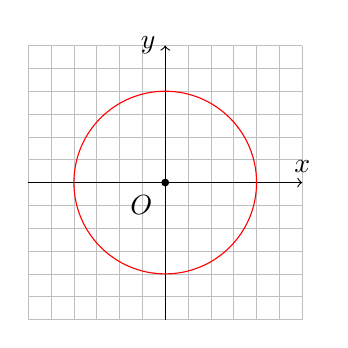
\begin{tikzpicture}[scale=0.29]
      \draw[very thin, lightgray] (-6,-6) grid (6,6) ;
      \draw[thin,->] (-6,0)--(6,0) node[above]{$x$} ;
      \draw[thin,->] (0,-6)--(0,6) node[left]{$y$} ;
      \node[fill=black,inner sep=1pt,shape=circle,label=225:$O$] %
      (O) at (0,0) {} ;
      \draw[color=red] (0,0) circle (4) ;
    \end{tikzpicture}
  }
  \end{columns}
\end{frame}

% EJD: use numbers in example?
\begin{frame}
  \frametitle{Circles about Any Given Center}
  \begin{columns}
  \column{0.65\textwidth}
  \begin{itemize}[<+->]
  \item Similarly, the circle centered at $(a,b)$ of radius $r$ 
    is the set of all points at distance $r$ from $(a,b)$.
  \item Such a circle has equation
    \begin{equation*}
      \sqrt{(x-a)^2+(y-b)^2} = r
    \end{equation*}
  \item Simplifying,
    \begin{equation*}
      (x-a)^2+(y-b)^2 = r^2
    \end{equation*}
  \end{itemize}
  \column{0.35\textwidth}
  \only<1->{ %
    \centering
    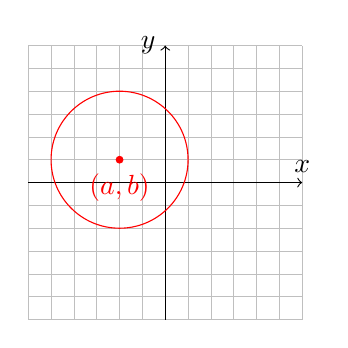
\begin{tikzpicture}[scale=0.29]
      \draw[very thin, lightgray] (-6,-6) grid (6,6) ;
      \draw[thin,->] (-6,0)--(6,0) node[above]{$x$} ;
      \draw[thin,->] (0,-6)--(0,6) node[left]{$y$} ;
      %\node[fill=black,inner sep=1pt,shape=circle,label=225:$O$] %
      %(O) at (0,0) {} ;
      \draw[red] (-2,1) circle (3) ;
      \node[fill=red,inner sep=1pt,shape=circle,label={[red]270:$(a,b)$}] %
      (A) at (-2,1) {} ;
    \end{tikzpicture}
  }
  \end{columns}
\end{frame}

% EJD: move these two/several slides to ``shifting conics''?
\begin{frame}
  \frametitle{Expanding an Equation of a Circle}
  \begin{columns}
  \column{0.65\textwidth}
  \begin{itemize}[<+->]
  \item Consider a circle centered at $(-2,1)$ of radius $3$.
    \begin{equation*}
      (x+2)^2 + (y-1)^2 = 3^2
    \end{equation*}
  \item We can expand to obtain
    \begin{equation*}
      x^2 +4x + 4 + y^2 -2y + 1 = 9
    \end{equation*}
  \item Moving constants, another way to write the equation of that
    circle is 
    \begin{equation*}
      x^2 + y^2 +4x-2y= 4
    \end{equation*}
  \end{itemize}
  \column{0.35\textwidth}
  % EJD: picture of the circle for decoration
  \only<1->{ %
    \centering
    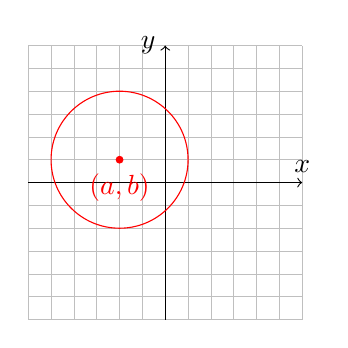
\begin{tikzpicture}[scale=0.29]
      \draw[very thin, lightgray] (-6,-6) grid (6,6) ;
      \draw[thin,->] (-6,0)--(6,0) node[above]{$x$} ;
      \draw[thin,->] (0,-6)--(0,6) node[left]{$y$} ;
      %\node[fill=black,inner sep=1pt,shape=circle,label=225:$O$] %
      %(O) at (0,0) {} ;
      \draw[red] (-2,1) circle (3) ;
      \node[fill=red,inner sep=1pt,shape=circle,label={[red]270:$(a,b)$}] %
      (A) at (-2,1) {} ;
    \end{tikzpicture}
  }
  \end{columns}
\end{frame}

\begin{frame}
  \frametitle{Completing the Square}
  \begin{columns}
  \column{0.65\textwidth}
  \begin{itemize}[<+->]
  \item<1-> On the other hand, sometimes we are given a circle in expanded
    form and must determine its center and radius.
  \item<2-> For example: $x^2+y^2-4x+2y=11$
  \item<3-> Put the $x$'s together: $x^2-4x+y^2+2y=11$
  \item<4-> Complete the square
    \begin{align*}
      x^2-4x+4 + y^2 +2y + 1 &= 11 + 4 + 1 \\
      (x-2)^2 + (y+1)^2 &= 16 = 4^2
    \end{align*}
  \item<5-> The circle has center $(2,-1)$ and radius $4$
  \end{itemize}
  \column{0.35\textwidth}
  % EJD: picture of the circle for decoration
  \only<1-4>{ %
    \centering
    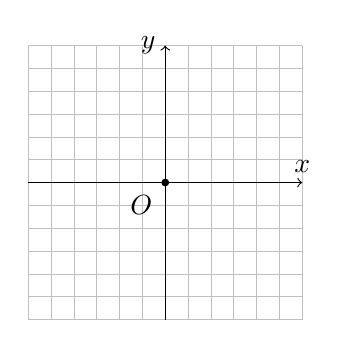
\begin{tikzpicture}[scale=0.29]
      \draw[very thin, lightgray] (-6,-6) grid (6,6) ;
      \draw[thin,->] (-6,0)--(6,0) node[above]{$x$} ;
      \draw[thin,->] (0,-6)--(0,6) node[left]{$y$} ;
      \node[fill=black,inner sep=1pt,shape=circle,label=225:$O$] %
      (O) at (0,0) {} ;
      %\node[fill=black,inner sep=1pt,shape=circle,label=225:$O$] %
      %(O) at (0,0) {} ;
      %\draw[red] (2,-1) circle (4) ;
      %\node[fill=red,inner sep=1pt,shape=circle,label={[red]270:$(2,-1)$}] %
      %(A) at (2,-1) {} ;
    \end{tikzpicture}
  }
  \only<5>{ %
    \centering
    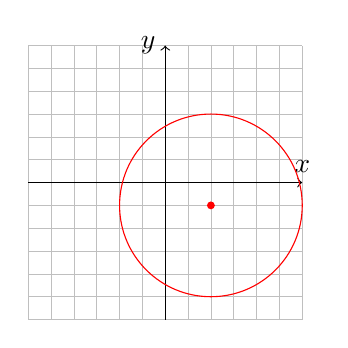
\begin{tikzpicture}[scale=0.29]
      \draw[very thin, lightgray] (-6,-6) grid (6,6) ;
      \draw[thin,->] (-6,0)--(6,0) node[above]{$x$} ;
      \draw[thin,->] (0,-6)--(0,6) node[left]{$y$} ;
      %\node[fill=black,inner sep=1pt,shape=circle,label=225:$O$] %
      %(O) at (0,0) {} ;
      \draw[red] (2,-1) circle (4) ;
      \node[fill=red,inner sep=1pt,shape=circle] %
      (A) at (2,-1) {} ;
    \end{tikzpicture}
  }
  \end{columns}
\end{frame}


\subsection{Parabolas}

% EJD: change height of graph from -6 .. 6 to -10..10 throughout!!
\begin{frame}
  \frametitle{Plotting Points}
  \begin{columns}
  \column{0.65\textwidth}
  \begin{itemize}[<+->]
  \item Another type of quadratic we may encounter is like:
    $2x^2-y=0$
  \item This time we can solve for $y$:
    \begin{equation*}
      2x^2 = y
    \end{equation*}
  \item So we can pick values for $x$ and get a corresponding value
    for $y$.
    % EJD: table or maybe \only<?>
  \item When $x=0$, $y=0$; when $x=1$, $y=2$; etc.
  \item Connect the dots smoothly to get the curve.
  \end{itemize}
  \column{0.35\textwidth}
  % EJD: picture with plotted points
  \only<1-3>{ %
    \centering
    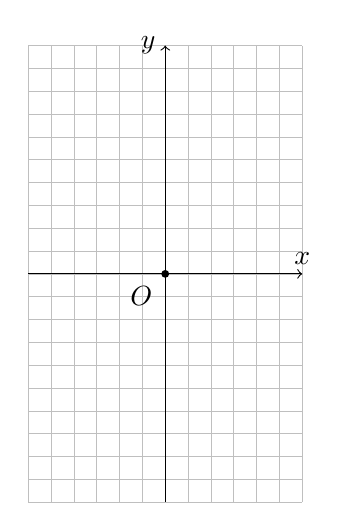
\begin{tikzpicture}[scale=0.29]
      \draw[very thin, lightgray] (-6,-10) grid (6,10) ;
      \draw[thin,->] (-6,0)--(6,0) node[above]{$x$} ;
      \draw[thin,->] (0,-10)--(0,10) node[left]{$y$} ;
      \node[fill=black,inner sep=1pt,shape=circle,label=225:$O$] %
      (O) at (0,0) {} ;
    \end{tikzpicture}
  }
  \only<4>{ %
    \centering
    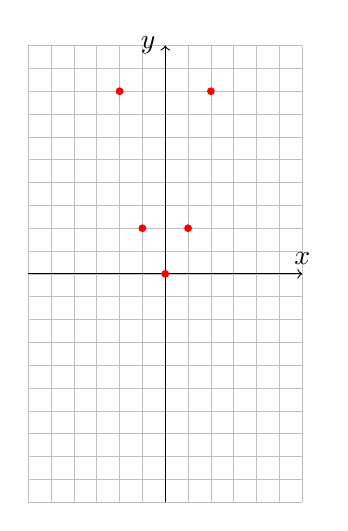
\begin{tikzpicture}[scale=0.29]
      \draw[very thin, lightgray] (-6,-10) grid (6,10) ;
      \draw[thin,->] (-6,0)--(6,0) node[above]{$x$} ;
      \draw[thin,->] (0,-10)--(0,10) node[left]{$y$} ;
      %\node[fill=black,inner sep=1pt,shape=circle,label=225:$O$] %
      %(O) at (0,0) {} ;
      \node[fill=red,inner sep=1pt,shape=circle] (P1) at (0,0) {} ;
      \node[fill=red,inner sep=1pt,shape=circle] (P2) at (1,2) {} ;
      \node[fill=red,inner sep=1pt,shape=circle] (P3) at (-1,2) {} ;
      \node[fill=red,inner sep=1pt,shape=circle] (P4) at (2,8) {} ;
      \node[fill=red,inner sep=1pt,shape=circle] (P5) at (-2,8) {} ;
    \end{tikzpicture}
  }
  \only<5->{ %
    \centering
    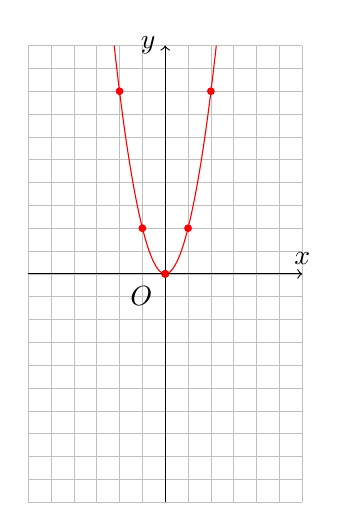
\begin{tikzpicture}[scale=0.29]
      \draw[very thin, lightgray] (-6,-10) grid (6,10) ;
      \draw[thin,->] (-6,0)--(6,0) node[above]{$x$} ;
      \draw[thin,->] (0,-10)--(0,10) node[left]{$y$} ;
      \node[fill=black,inner sep=1pt,shape=circle,label=225:$O$] %
      (O) at (0,0) {} ;
      \node[fill=red,inner sep=1pt,shape=circle] (P1) at (0,0) {} ;
      \node[fill=red,inner sep=1pt,shape=circle] (P2) at (1,2) {} ;
      \node[fill=red,inner sep=1pt,shape=circle] (P3) at (-1,2) {} ;
      \node[fill=red,inner sep=1pt,shape=circle] (P4) at (2,8) {} ;
      \node[fill=red,inner sep=1pt,shape=circle] (P5) at (-2,8) {} ;
      \draw[red] (0,0) parabola ({sqrt(5)},10) ;
      \draw[red] (0,0) parabola ({-sqrt(5)},10) ;
    \end{tikzpicture}
  }
  \end{columns}
\end{frame}

\begin{frame}
  \frametitle{Opening Upward/Downward}
  \begin{columns}
  \column{0.65\textwidth}
  \begin{itemize}[<+->]
  \item<1-> We can accelerate the process of graphing a parabola
    $y=ax^2$ if we note three things:
  \item<2-> Whether it opens upward ($a>0$) \only<3->{or downward
    ($a<0$)}
  \item<4-> Its vertex is always $(0,0)$
  \item<6-> It is symmetric about the $y$-axis
  \item<9-> With those observations we can get the general shape of the
    parabola.
  \item<10-> With one more point, we can get the exact shape of the
    parabola.
    % EJD: parabolas?  At least one graph
  \end{itemize}
  \column{0.35\textwidth}
  \only<1>{ %
    \centering
    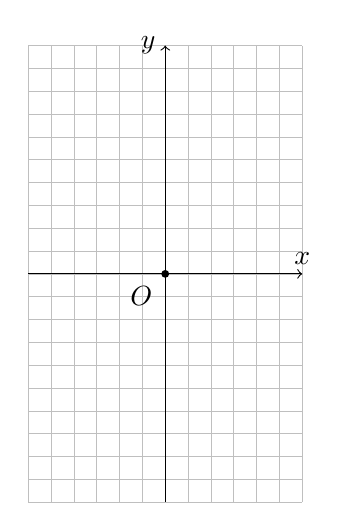
\begin{tikzpicture}[scale=0.29]
      \draw[very thin, lightgray] (-6,-10) grid (6,10) ;
      \draw[thin,->] (-6,0)--(6,0) node[above]{$x$} ;
      \draw[thin,->] (0,-10)--(0,10) node[left]{$y$} ;
      \node[fill=black,inner sep=1pt,shape=circle,label=225:$O$] %
      (O) at (0,0) {} ;
    \end{tikzpicture}
  }
  \only<2>{ %
    \centering
    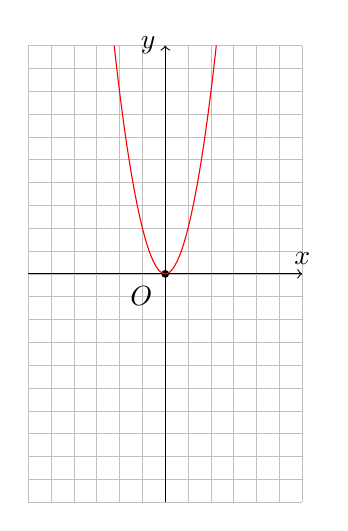
\begin{tikzpicture}[scale=0.29]
      \draw[very thin, lightgray] (-6,-10) grid (6,10) ;
      \draw[thin,->] (-6,0)--(6,0) node[above]{$x$} ;
      \draw[thin,->] (0,-10)--(0,10) node[left]{$y$} ;
      \node[fill=black,inner sep=1pt,shape=circle,label=225:$O$] %
      (O) at (0,0) {} ;
      \draw[red] (0,0) parabola ({-sqrt(5)},10) ;
      \draw[red] (0,0) parabola ({sqrt(5)},10) ;
    \end{tikzpicture}
  }
  \only<3>{ %
    \centering
    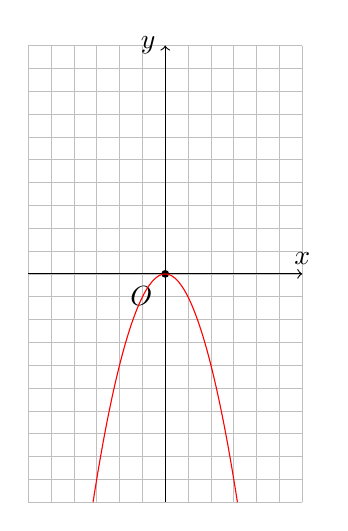
\begin{tikzpicture}[scale=0.29]
      \draw[very thin, lightgray] (-6,-10) grid (6,10) ;
      \draw[thin,->] (-6,0)--(6,0) node[above]{$x$} ;
      \draw[thin,->] (0,-10)--(0,10) node[left]{$y$} ;
      \node[fill=black,inner sep=1pt,shape=circle,label=225:$O$] %
      (O) at (0,0) {} ;
      \draw[red] (0,0) parabola ({-sqrt(10)},-10) ;
      \draw[red] (0,0) parabola ({sqrt(10)},-10) ;
    \end{tikzpicture}
  }
  \only<4>{ %
    \centering
    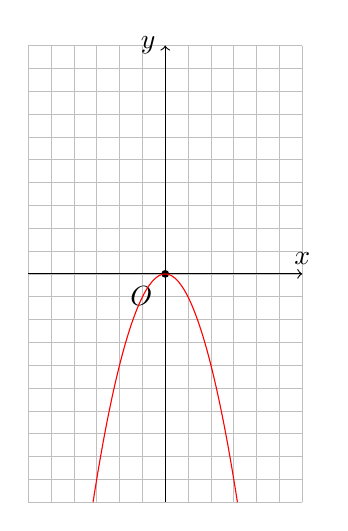
\begin{tikzpicture}[scale=0.29]
      \draw[very thin, lightgray] (-6,-10) grid (6,10) ;
      \draw[thin,->] (-6,0)--(6,0) node[above]{$x$} ;
      \draw[thin,->] (0,-10)--(0,10) node[left]{$y$} ;
      \node[fill=black,inner sep=1pt,shape=circle,label=225:$O$] %
      (O) at (0,0) {} ;
      \draw[red] (0,0) parabola ({-sqrt(10)},-10) ;
      \draw[red] (0,0) parabola ({sqrt(10)},-10) ;
    \end{tikzpicture}
  }
  \only<5>{ %
    \centering
    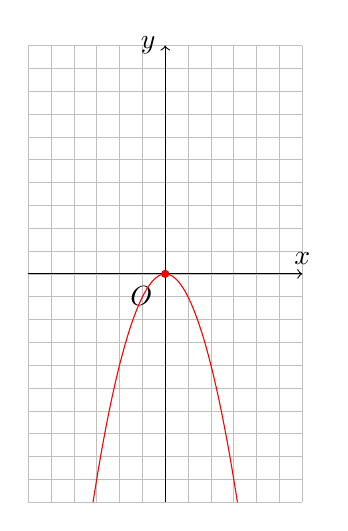
\begin{tikzpicture}[scale=0.29]
      \draw[very thin, lightgray] (-6,-10) grid (6,10) ;
      \draw[thin,->] (-6,0)--(6,0) node[above]{$x$} ;
      \draw[thin,->] (0,-10)--(0,10) node[left]{$y$} ;
      \node[fill=black,inner sep=1pt,shape=circle,label=225:$O$] %
      (O) at (0,0) {} ;
      \draw[red] (0,0) parabola ({-sqrt(10)},-10) ;
      \draw[red] (0,0) parabola ({sqrt(10)},-10) ;
      \node[fill=red,inner sep=1pt,shape=circle] (V) at (0,0) {} ;
    \end{tikzpicture}
  }
  \only<6>{ %
    \centering
    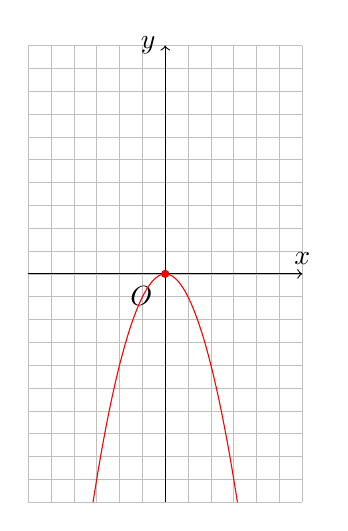
\begin{tikzpicture}[scale=0.29]
      \draw[very thin, lightgray] (-6,-10) grid (6,10) ;
      \draw[thin,->] (-6,0)--(6,0) node[above]{$x$} ;
      \draw[thin,->] (0,-10)--(0,10) node[left]{$y$} ;
      \node[fill=black,inner sep=1pt,shape=circle,label=225:$O$] %
      (O) at (0,0) {} ;
      \draw[red] (0,0) parabola ({-sqrt(10)},-10) ;
      \draw[red] (0,0) parabola ({sqrt(10)},-10) ;
      \node[fill=red,inner sep=1pt,shape=circle] (V) at (0,0) {} ;
    \end{tikzpicture}
  }
  \only<7>{ %
    \centering
    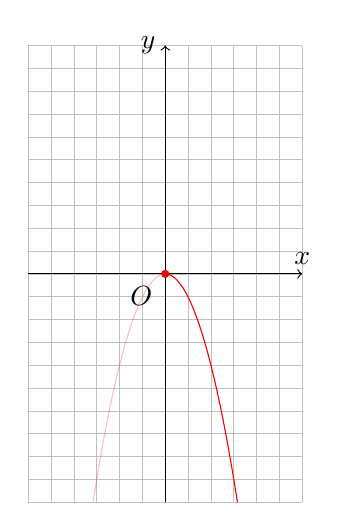
\begin{tikzpicture}[scale=0.29]
      \draw[very thin, lightgray] (-6,-10) grid (6,10) ;
      \draw[thin,->] (-6,0)--(6,0) node[above]{$x$} ;
      \draw[thin,->] (0,-10)--(0,10) node[left]{$y$} ;
      \node[fill=black,inner sep=1pt,shape=circle,label=225:$O$] %
      (O) at (0,0) {} ;
      \draw[red,nearly transparent] (0,0) parabola ({-sqrt(10)},-10) ;
      \draw[red] (0,0) parabola ({sqrt(10)},-10) ;
      \node[fill=red,inner sep=1pt,shape=circle] (V) at (0,0) {} ;
    \end{tikzpicture}
  }
  \only<8>{ %
    \centering
    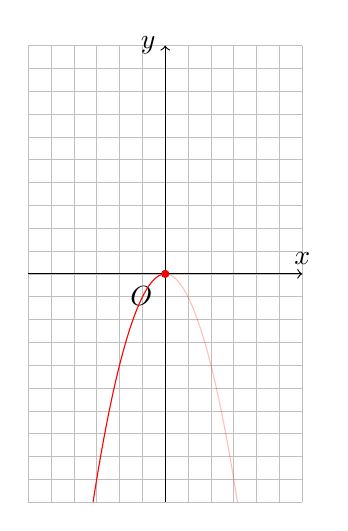
\begin{tikzpicture}[scale=0.29]
      \draw[very thin, lightgray] (-6,-10) grid (6,10) ;
      \draw[thin,->] (-6,0)--(6,0) node[above]{$x$} ;
      \draw[thin,->] (0,-10)--(0,10) node[left]{$y$} ;
      \node[fill=black,inner sep=1pt,shape=circle,label=225:$O$] %
      (O) at (0,0) {} ;
      \draw[red] (0,0) parabola ({-sqrt(10)},-10) ;
      \draw[red,nearly transparent] (0,0) parabola ({sqrt(10)},-10) ;
      \node[fill=red,inner sep=1pt,shape=circle] (V) at (0,0) {} ;
    \end{tikzpicture}
  }
  \only<9>{ %
    \centering
    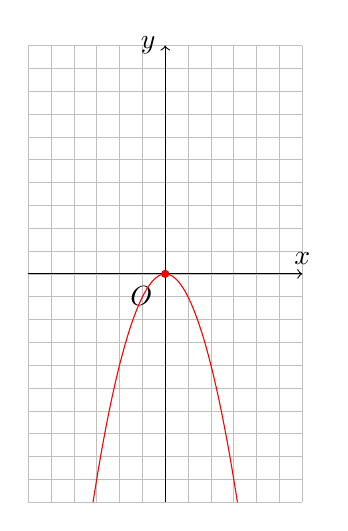
\begin{tikzpicture}[scale=0.29]
      \draw[very thin, lightgray] (-6,-10) grid (6,10) ;
      \draw[thin,->] (-6,0)--(6,0) node[above]{$x$} ;
      \draw[thin,->] (0,-10)--(0,10) node[left]{$y$} ;
      \node[fill=black,inner sep=1pt,shape=circle,label=225:$O$] %
      (O) at (0,0) {} ;
      \draw[red] (0,0) parabola ({-sqrt(10)},-10) ;
      \draw[red] (0,0) parabola ({sqrt(10)},-10) ;
      \node[fill=red,inner sep=1pt,shape=circle] (V) at (0,0) {} ;
    \end{tikzpicture}
  }
  \only<10>{ %
    \centering
    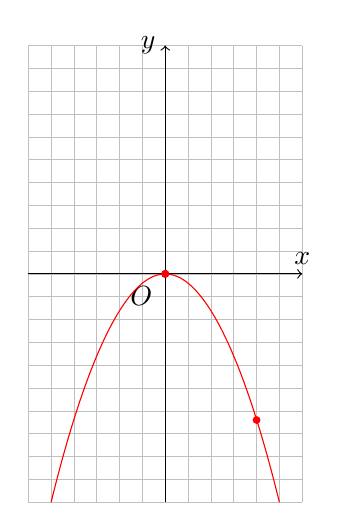
\begin{tikzpicture}[scale=0.29]
      \draw[very thin, lightgray] (-6,-10) grid (6,10) ;
      \draw[thin,->] (-6,0)--(6,0) node[above]{$x$} ;
      \draw[thin,->] (0,-10)--(0,10) node[left]{$y$} ;
      \node[fill=black,inner sep=1pt,shape=circle,label=225:$O$] %
      (O) at (0,0) {} ;
      \draw[red] (0,0) parabola (-5,-10) ;
      \draw[red] (0,0) parabola (5,-10) ;
      \node[fill=red,inner sep=1pt,shape=circle] (V) at (0,0) {} ;
      \node[fill=red,inner sep=1pt,shape=circle] (P) at (4,-6.4) {} ;
    \end{tikzpicture}
  }
  \end{columns}
\end{frame}

%% \begin{frame}
%%   \frametitle{Symmetry Properties}
%%   \begin{columns}
%%   \column{0.65\textwidth}
%%   \begin{itemize}[<-+>]
%%   \item X
%%   \end{itemize}
%%   \column{0.35\textwidth}
%%   \end{columns}
%% \end{frame}

\begin{frame}
  \frametitle{Opening Left/Right}
  \begin{columns}
  \column{0.65\textwidth}
  \begin{itemize}[<+->]
  \item<1-> Similarly, we can graph any parabola of the form $x=ay^2$
  \item<2-> We can accelerate the process if we note three things:
  \item<3-> Whether it opens to the right ($a>0$) \only<4->{or to the left
    ($a<0$)}
  \item<5-> Its vertex is always $(0,0)$
  \item<7-> It is symmetric about the $x$-axis
  \item<10-> With those observations we can get the general shape of the
    parabola.
  \item<11-> With one more point, we can get the exact shape of the
    parabola.
    % EJD: parabolas?  At least one graph
  \end{itemize}
  \column{0.35\textwidth}
  \only<1-2>{ %
    \centering
    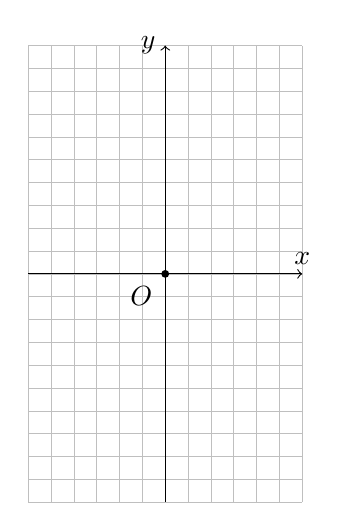
\begin{tikzpicture}[scale=0.29]
      \draw[very thin, lightgray] (-6,-10) grid (6,10) ;
      \draw[thin,->] (-6,0)--(6,0) node[above]{$x$} ;
      \draw[thin,->] (0,-10)--(0,10) node[left]{$y$} ;
      \node[fill=black,inner sep=1pt,shape=circle,label=225:$O$] %
      (O) at (0,0) {} ;
    \end{tikzpicture}
  }
  \only<3>{ %
    \centering
    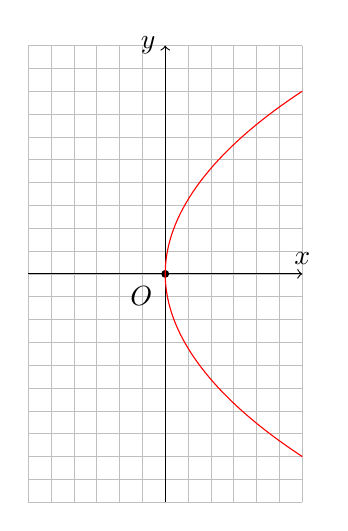
\begin{tikzpicture}[scale=0.29]
      \draw[very thin, lightgray] (-6,-10) grid (6,10) ;
      \draw[thin,->] (-6,0)--(6,0) node[above]{$x$} ;
      \draw[thin,->] (0,-10)--(0,10) node[left]{$y$} ;
      \node[fill=black,inner sep=1pt,shape=circle,label=225:$O$] %
      (O) at (0,0) {} ;
      \draw[red,rotate=-90] (0,0) parabola (8,6) ;
      \draw[red,rotate=-90] (0,0) parabola (-8,6) ;
    \end{tikzpicture}
  }
  \only<4>{ %
    \centering
    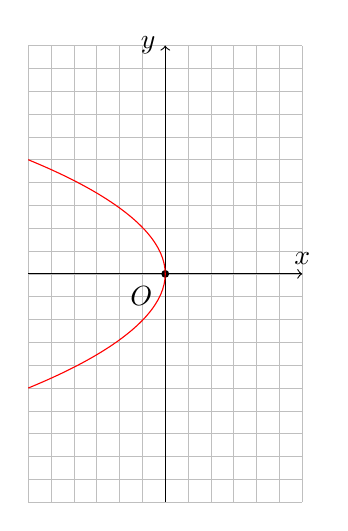
\begin{tikzpicture}[scale=0.29]
      \draw[very thin, lightgray] (-6,-10) grid (6,10) ;
      \draw[thin,->] (-6,0)--(6,0) node[above]{$x$} ;
      \draw[thin,->] (0,-10)--(0,10) node[left]{$y$} ;
      \node[fill=black,inner sep=1pt,shape=circle,label=225:$O$] %
      (O) at (0,0) {} ;
      \draw[red,rotate=-90] (0,0) parabola (5,-6) ;
      \draw[red,rotate=-90] (0,0) parabola (-5,-6) ;
    \end{tikzpicture}
  }
  \only<5>{ %
    \centering
    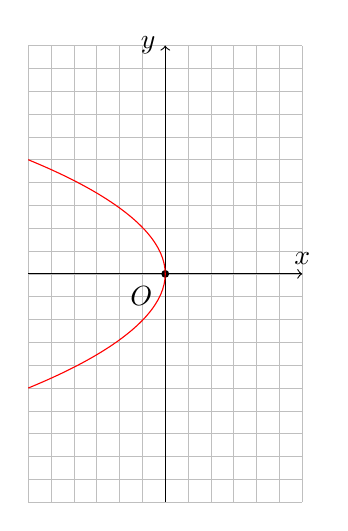
\begin{tikzpicture}[scale=0.29]
      \draw[very thin, lightgray] (-6,-10) grid (6,10) ;
      \draw[thin,->] (-6,0)--(6,0) node[above]{$x$} ;
      \draw[thin,->] (0,-10)--(0,10) node[left]{$y$} ;
      \node[fill=black,inner sep=1pt,shape=circle,label=225:$O$] %
      (O) at (0,0) {} ;
      \draw[red,rotate=-90] (0,0) parabola (5,-6) ;
      \draw[red,rotate=-90] (0,0) parabola (-5,-6) ;
    \end{tikzpicture}
  }
  \only<6>{ %
    \centering
    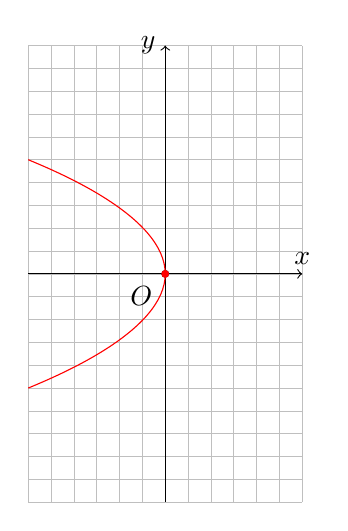
\begin{tikzpicture}[scale=0.29]
      \draw[very thin, lightgray] (-6,-10) grid (6,10) ;
      \draw[thin,->] (-6,0)--(6,0) node[above]{$x$} ;
      \draw[thin,->] (0,-10)--(0,10) node[left]{$y$} ;
      \node[fill=black,inner sep=1pt,shape=circle,label=225:$O$] %
      (O) at (0,0) {} ;
      \draw[red,rotate=-90] (0,0) parabola (5,-6) ;
      \draw[red,rotate=-90] (0,0) parabola (-5,-6) ;
      \node[fill=red,inner sep=1pt,shape=circle] (V) at (0,0) {} ;
    \end{tikzpicture}
  }
  \only<7>{ %
    \centering
    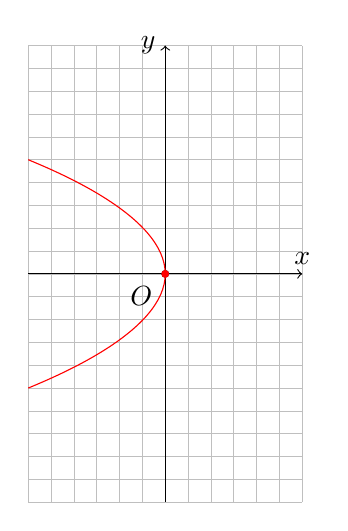
\begin{tikzpicture}[scale=0.29]
      \draw[very thin, lightgray] (-6,-10) grid (6,10) ;
      \draw[thin,->] (-6,0)--(6,0) node[above]{$x$} ;
      \draw[thin,->] (0,-10)--(0,10) node[left]{$y$} ;
      \node[fill=black,inner sep=1pt,shape=circle,label=225:$O$] %
      (O) at (0,0) {} ;
      \draw[red,rotate=-90] (0,0) parabola (5,-6) ;
      \draw[red,rotate=-90] (0,0) parabola (-5,-6) ;
      \node[fill=red,inner sep=1pt,shape=circle] (V) at (0,0) {} ;
    \end{tikzpicture}
  }
  \only<8>{ %
    \centering
    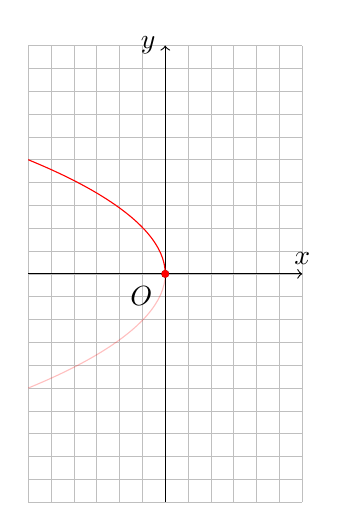
\begin{tikzpicture}[scale=0.29]
      \draw[very thin, lightgray] (-6,-10) grid (6,10) ;
      \draw[thin,->] (-6,0)--(6,0) node[above]{$x$} ;
      \draw[thin,->] (0,-10)--(0,10) node[left]{$y$} ;
      \node[fill=black,inner sep=1pt,shape=circle,label=225:$O$] %
      (O) at (0,0) {} ;
      \draw[red,nearly transparent,rotate=-90] (0,0) parabola (5,-6) ;
      \draw[red,rotate=-90] (0,0) parabola (-5,-6) ;
      \node[fill=red,inner sep=1pt,shape=circle] (V) at (0,0) {} ;
    \end{tikzpicture}
  }
  \only<9>{ %
    \centering
    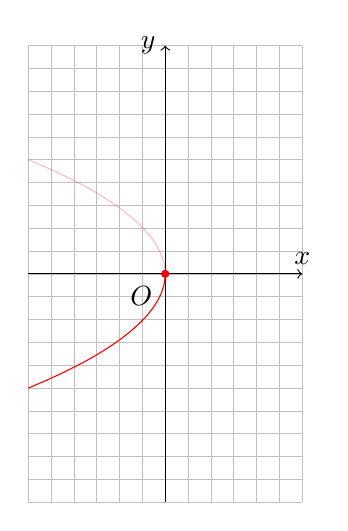
\begin{tikzpicture}[scale=0.29]
      \draw[very thin, lightgray] (-6,-10) grid (6,10) ;
      \draw[thin,->] (-6,0)--(6,0) node[above]{$x$} ;
      \draw[thin,->] (0,-10)--(0,10) node[left]{$y$} ;
      \node[fill=black,inner sep=1pt,shape=circle,label=225:$O$] %
      (O) at (0,0) {} ;
      \draw[red,rotate=-90] (0,0) parabola (5,-6) ;
      \draw[red,nearly transparent,rotate=-90] (0,0) parabola (-5,-6) ;
      \node[fill=red,inner sep=1pt,shape=circle] (V) at (0,0) {} ;
    \end{tikzpicture}
  }
  \only<10>{ %
    \centering
    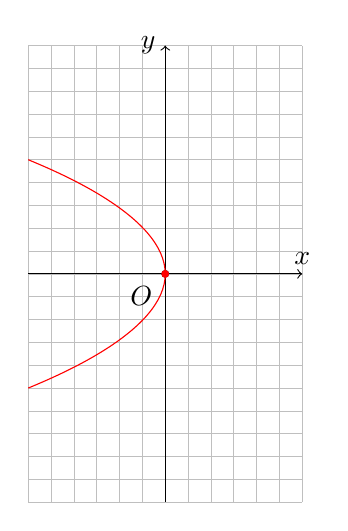
\begin{tikzpicture}[scale=0.29]
      \draw[very thin, lightgray] (-6,-10) grid (6,10) ;
      \draw[thin,->] (-6,0)--(6,0) node[above]{$x$} ;
      \draw[thin,->] (0,-10)--(0,10) node[left]{$y$} ;
      \node[fill=black,inner sep=1pt,shape=circle,label=225:$O$] %
      (O) at (0,0) {} ;
      \draw[red,rotate=-90] (0,0) parabola (5,-6) ;
      \draw[red,rotate=-90] (0,0) parabola (-5,-6) ;
      \node[fill=red,inner sep=1pt,shape=circle] (V) at (0,0) {} ;
    \end{tikzpicture}
  }
  \only<11>{ %
    \centering
    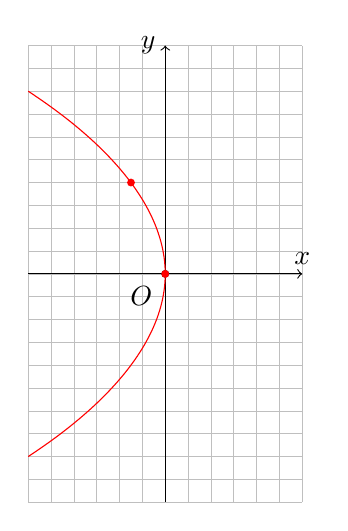
\begin{tikzpicture}[scale=0.29]
      \draw[very thin, lightgray] (-6,-10) grid (6,10) ;
      \draw[thin,->] (-6,0)--(6,0) node[above]{$x$} ;
      \draw[thin,->] (0,-10)--(0,10) node[left]{$y$} ;
      \node[fill=black,inner sep=1pt,shape=circle,label=225:$O$] %
      (O) at (0,0) {} ;
      \draw[red,rotate=-90] (0,0) parabola (-8,-6) ;
      \draw[red,rotate=-90] (0,0) parabola (8,-6) ;
      \node[fill=red,inner sep=1pt,shape=circle] (V) at (0,0) {} ;
      \node[fill=red,inner sep=1pt,shape=circle] (P) at (-1.5,4) {} ;
    \end{tikzpicture}
  }
  \end{columns}
\end{frame}

\begin{frame}
  \frametitle{Intersection between Line and Parabola}
  \begin{columns}
  \column{0.65\textwidth}
  \begin{itemize}[<+->]
  \item We will need to graph lines and parabolas on the same graph.
  \item When we do that we should find their intersection points.
  \item Suppose our line is $y=2-x$ and our parabola is $y=x^2$
  \item Eliminate $y$: $2-x=x^2$
  \item Solve: $x^2+x-2=0$ implies $(x+2)(x-1)=0$ so $x=-2$ or $x=1$
  \item Use $y=2-x$ to figure out the corresponding $y$-values: $y=4$
    or $y=1$
  \item The intersections are $(-2,4)$ and $(1,1)$
  \end{itemize}
  \column{0.35\textwidth}
  \only<1-2>{ %
    \centering
    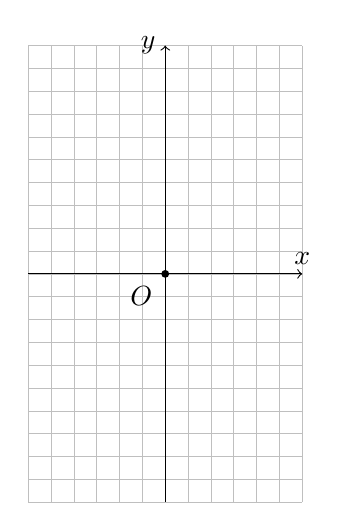
\begin{tikzpicture}[scale=0.29]
      \draw[very thin, lightgray] (-6,-10) grid (6,10) ;
      \draw[thin,->] (-6,0)--(6,0) node[above]{$x$} ;
      \draw[thin,->] (0,-10)--(0,10) node[left]{$y$} ;
      \node[fill=black,inner sep=1pt,shape=circle,label=225:$O$] %
      (O) at (0,0) {} ;
    \end{tikzpicture}
  }
  \only<3-6>{ % Maybe add lines to show determination of x-val, just
              % show line not parabola to show det. of y-val
    \centering
    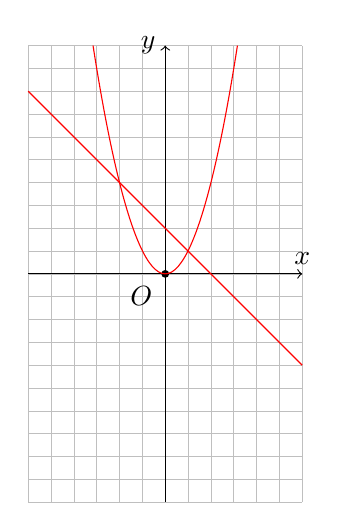
\begin{tikzpicture}[scale=0.29]
      \draw[very thin, lightgray] (-6,-10) grid (6,10) ;
      \draw[thin,->] (-6,0)--(6,0) node[above]{$x$} ;
      \draw[thin,->] (0,-10)--(0,10) node[left]{$y$} ;
      \node[fill=black,inner sep=1pt,shape=circle,label=225:$O$] %
      (O) at (0,0) {} ;
      \draw[red] (-6,8)--(6,-4) ;
      \draw[red] (0,0) parabola ({sqrt(10)},10) ;
      \draw[red] (0,0) parabola ({-sqrt(10)},10) ;
    \end{tikzpicture}
  }
  \only<7->{ %
    \centering
    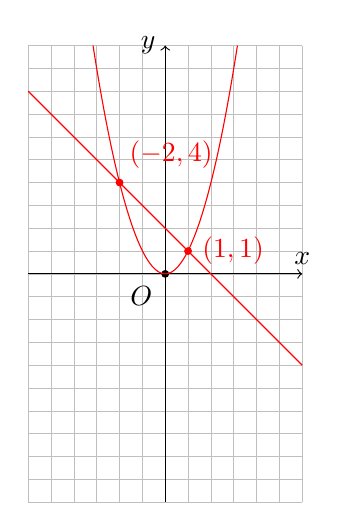
\begin{tikzpicture}[scale=0.29]
      \draw[very thin, lightgray] (-6,-10) grid (6,10) ;
      \draw[thin,->] (-6,0)--(6,0) node[above]{$x$} ;
      \draw[thin,->] (0,-10)--(0,10) node[left]{$y$} ;
      \node[fill=black,inner sep=1pt,shape=circle,label=225:$O$] %
      (O) at (0,0) {} ;
      \draw[red] (-6,8)--(6,-4) ;
      \draw[red] (0,0) parabola ({sqrt(10)},10) ;
      \draw[red] (0,0) parabola ({-sqrt(10)},10) ;
      \node[fill=red,inner sep=1pt,shape=circle,label={[red]86:$(-2,4)$}] %
      (A) at (-2,4) {} ;
      \node[fill=red,inner sep=1pt,shape=circle,label={[red]0:$(1,1)$}] %
      (B) at (1,1) {} ;
    \end{tikzpicture}
  }
  \end{columns}
\end{frame}


\subsection{Ellipses and Hyperbolas}

\begin{frame}
  \frametitle{Ellipses Centered at $(0,0)$}
  \begin{columns}
  \column{0.65\textwidth}
  \begin{itemize}[<+->]
  \item<1-> An ellipse is a ``flattened circle''.
  \item<2-> Start with a unit circle centered at $(0,0)$:
    \begin{equation*}
      x^2 + y^2 = 1
    \end{equation*}
  \item<3-> Scale the $x$ and $y$ variables separately:
    \begin{equation*}
      \left(\frac{x}{a}\right)^2 + \left(\frac{y}{b}\right)^2 = 1
    \end{equation*}
  \item<6-> The equation is usually written 
    \begin{equation*}
      \frac{x^2}{a^2} + \frac{y^2}{b^2} = 1
    \end{equation*}
  \end{itemize}
  \column{0.35\textwidth}
  \only<1>{ %
    \centering
    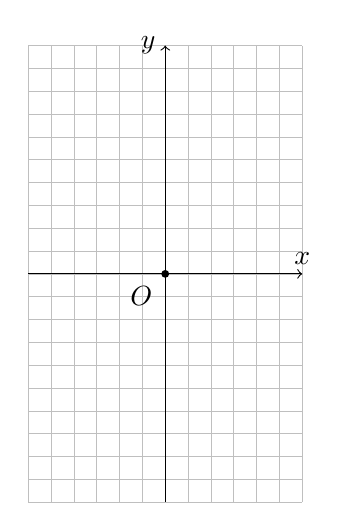
\begin{tikzpicture}[scale=0.29]
      \draw[very thin, lightgray] (-6,-10) grid (6,10) ;
      \draw[thin,->] (-6,0)--(6,0) node[above]{$x$} ;
      \draw[thin,->] (0,-10)--(0,10) node[left]{$y$} ;
      \node[fill=black,inner sep=1pt,shape=circle,label=225:$O$] %
      (O) at (0,0) {} ;
    \end{tikzpicture}
  }
  \only<2-3>{ %
    \centering
    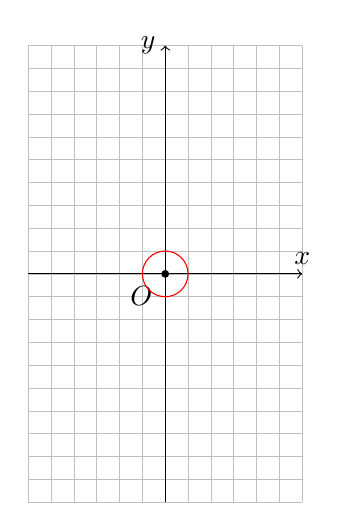
\begin{tikzpicture}[scale=0.29]
      \draw[very thin, lightgray] (-6,-10) grid (6,10) ;
      \draw[thin,->] (-6,0)--(6,0) node[above]{$x$} ;
      \draw[thin,->] (0,-10)--(0,10) node[left]{$y$} ;
      \node[fill=black,inner sep=1pt,shape=circle,label=225:$O$] %
      (O) at (0,0) {} ;
      \draw[red] (0,0) ellipse (1 and 1) ;
    \end{tikzpicture}
  }
  \only<4>{ %
    \centering
    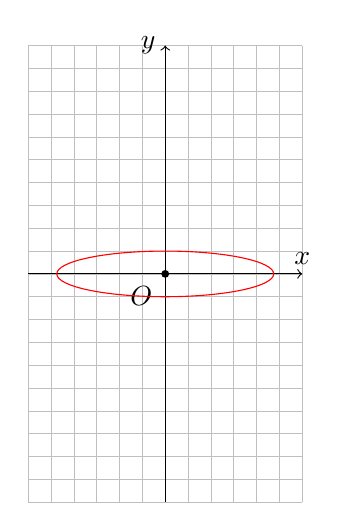
\begin{tikzpicture}[scale=0.29]
      \draw[very thin, lightgray] (-6,-10) grid (6,10) ;
      \draw[thin,->] (-6,0)--(6,0) node[above]{$x$} ;
      \draw[thin,->] (0,-10)--(0,10) node[left]{$y$} ;
      \node[fill=black,inner sep=1pt,shape=circle,label=225:$O$] %
      (O) at (0,0) {} ;
      \draw[red] (0,0) ellipse (4.75 and 1) ;
    \end{tikzpicture}
  }
  \only<5->{ %
    \centering
    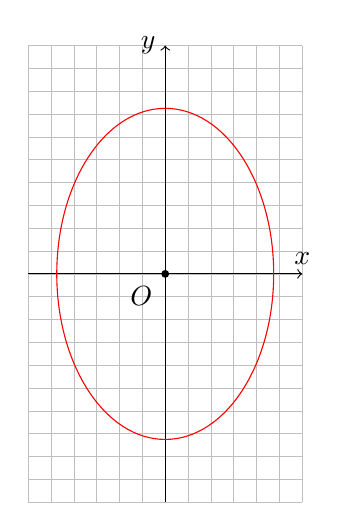
\begin{tikzpicture}[scale=0.29]
      \draw[very thin, lightgray] (-6,-10) grid (6,10) ;
      \draw[thin,->] (-6,0)--(6,0) node[above]{$x$} ;
      \draw[thin,->] (0,-10)--(0,10) node[left]{$y$} ;
      \node[fill=black,inner sep=1pt,shape=circle,label=225:$O$] %
      (O) at (0,0) {} ;
      \draw[red] (0,0) ellipse (4.75 and 7.25) ;
    \end{tikzpicture}
  }
  \end{columns}
\end{frame}

\begin{frame}
  \frametitle{Intercepts of an Ellipse}
  \begin{columns}
  \column{0.65\textwidth}
  \begin{itemize}[<+->]
  \item<1-> Recall the equation of an ellipse in standard position
    (centered at the origin):
    \begin{equation*}
      \frac{x^2}{a^2} + \frac{y^2}{b^2} = 1
    \end{equation*}
  \item<2-> If $x=0$, we get $y^2=b^2 \implies y=\pm b$
  \item<3-> So the $y$-intercepts are $(0,-b)$ and $(0,b)$
  \item<4-> Similarly the $x$-intercepts are $(-a,0)$ and $(a,0)$.
  \end{itemize}
  \column{0.35\textwidth}
  % EJD: graphs
  \only<1-2>{ %
    \centering
    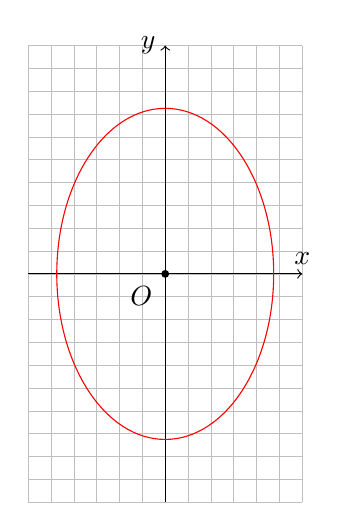
\begin{tikzpicture}[scale=0.29]
      \draw[very thin, lightgray] (-6,-10) grid (6,10) ;
      \draw[thin,->] (-6,0)--(6,0) node[above]{$x$} ;
      \draw[thin,->] (0,-10)--(0,10) node[left]{$y$} ;
      \node[fill=black,inner sep=1pt,shape=circle,label=225:$O$] %
      (O) at (0,0) {} ;
      \draw[red] (0,0) ellipse (4.75 and 7.25) ;
    \end{tikzpicture}
  }
  \only<3>{ %
    \centering
    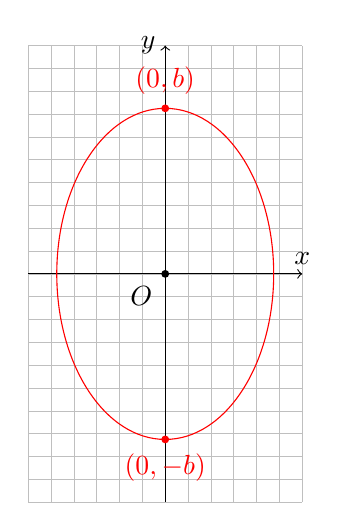
\begin{tikzpicture}[scale=0.29]
      \draw[very thin, lightgray] (-6,-10) grid (6,10) ;
      \draw[thin,->] (-6,0)--(6,0) node[above]{$x$} ;
      \draw[thin,->] (0,-10)--(0,10) node[left]{$y$} ;
      \node[fill=black,inner sep=1pt,shape=circle,label=225:$O$] %
      (O) at (0,0) {} ;
      \draw[red] (0,0) ellipse (4.75 and 7.25) ;
      \node[fill=red,inner sep=1pt,shape=circle,label={[red]270:$(0,-b)$}] %
      (I1) at (0,-7.25) {} ;
      \node[fill=red,inner sep=1pt,shape=circle,label={[red]90:$(0,b)$}] %
      (I2) at (0,7.25) {} ;
    \end{tikzpicture}
  }
  \only<4>{ %
    \centering
    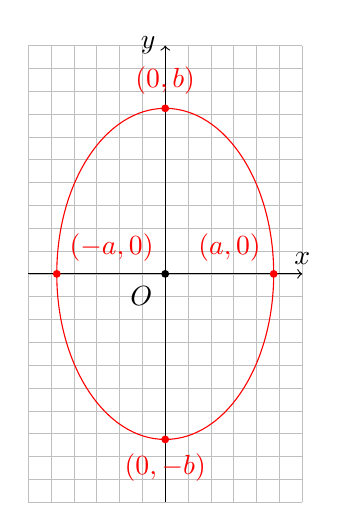
\begin{tikzpicture}[scale=0.29]
      \draw[very thin, lightgray] (-6,-10) grid (6,10) ;
      \draw[thin,->] (-6,0)--(6,0) node[above]{$x$} ;
      \draw[thin,->] (0,-10)--(0,10) node[left]{$y$} ;
      \node[fill=black,inner sep=1pt,shape=circle,label=225:$O$] %
      (O) at (0,0) {} ;
      \draw[red] (0,0) ellipse (4.75 and 7.25) ;
      \node[fill=red,inner sep=1pt,shape=circle,label={[red]270:$(0,-b)$}] %
      (I1) at (0,-7.25) {} ;
      \node[fill=red,inner sep=1pt,shape=circle,label={[red]90:$(0,b)$}] %
      (I2) at (0,7.25) {} ;
      \node[fill=red,inner sep=1pt,shape=circle,label={[red]45:$(-a,0)$}] %
      (I3) at (-4.75,0) {} ;
      \node[fill=red,inner sep=1pt,shape=circle,label={[red]135:$(a,0)$}] %
      (I4) at (4.75,0) {} ;
    \end{tikzpicture}
  }
  \end{columns}
\end{frame}

\begin{frame}
  \frametitle{Example: $9x^2+16y^2=144$}
  \begin{columns}
  \column{0.65\textwidth}
  \begin{itemize}[<+->]
  \item<1-> Consider the ellipse given by
    \begin{equation*}
      9x^2 + 16y^2 = 144
    \end{equation*}
  \item<2-> Dividing through by $144$ we have
    \begin{equation*}
      \frac{x^2}{16} + \frac{y^2}{9} = 1
    \end{equation*}
  \item<3-> By the method previous slide, the intercepts are $(0,-3)$,
    $(0,3)$, $(-4,0)$, $(4,0)$
  \item<4-> We can now draw a rough graph of the ellipse.
  \end{itemize}
  \column{0.35\textwidth}
  \only<1-2>{ %
    \centering
    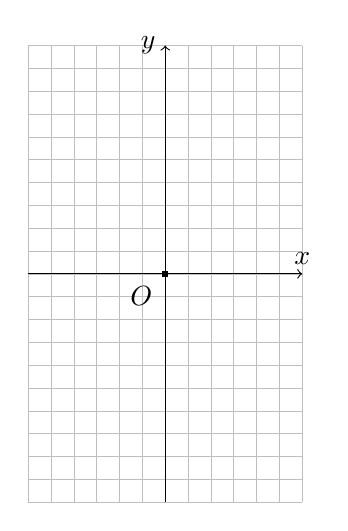
\begin{tikzpicture}[scale=0.29]
      \draw[very thin, lightgray] (-6,-10) grid (6,10) ;
      \draw[thin,->] (-6,0)--(6,0) node[above]{$x$} ;
      \draw[thin,->] (0,-10)--(0,10) node[left]{$y$} ;
      \node[fill=black,inner sep=1pt,label=225:$O$] (O) at (0,0) {} ;
    \end{tikzpicture}
  }
  \only<3>{ %
    \centering
    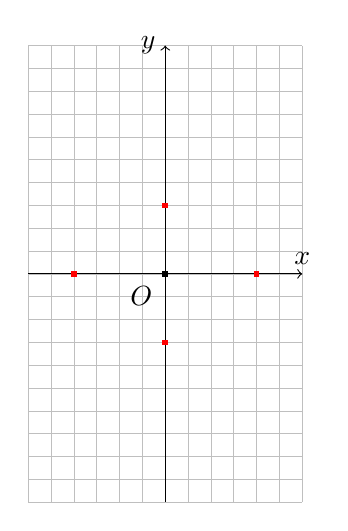
\begin{tikzpicture}[scale=0.29]
      \draw[very thin, lightgray] (-6,-10) grid (6,10) ;
      \draw[thin,->] (-6,0)--(6,0) node[above]{$x$} ;
      \draw[thin,->] (0,-10)--(0,10) node[left]{$y$} ;
      \node[fill=black,inner sep=1pt,label=225:$O$] (O) at (0,0) {} ;
      %\draw[red] (0,0) ellipse (4 and 3) ;
      \node[fill=red,inner sep=1pt] (I1) at (-4,0) {} ;
      \node[fill=red,inner sep=1pt] (I2) at (4,0) {} ;
      \node[fill=red,inner sep=1pt] (I3) at (0,-3) {} ;
      \node[fill=red,inner sep=1pt] (I4) at (0,3) {} ;
    \end{tikzpicture}
  }
  \only<4>{ %
    \centering
    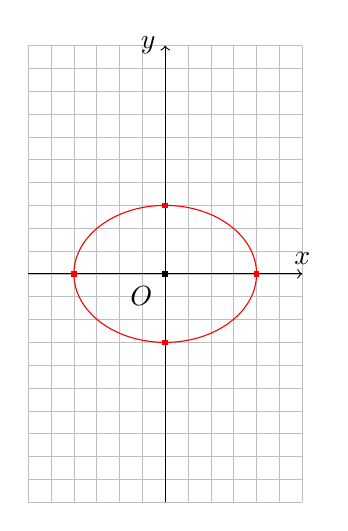
\begin{tikzpicture}[scale=0.29]
      \draw[very thin, lightgray] (-6,-10) grid (6,10) ;
      \draw[thin,->] (-6,0)--(6,0) node[above]{$x$} ;
      \draw[thin,->] (0,-10)--(0,10) node[left]{$y$} ;
      \node[fill=black,inner sep=1pt,label=225:$O$] (O) at (0,0) {} ;
      \draw[red] (0,0) ellipse (4 and 3) ;
      \node[fill=red,inner sep=1pt] (I1) at (-4,0) {} ;
      \node[fill=red,inner sep=1pt] (I2) at (4,0) {} ;
      \node[fill=red,inner sep=1pt] (I3) at (0,-3) {} ;
      \node[fill=red,inner sep=1pt] (I4) at (0,3) {} ;
    \end{tikzpicture}
  } % EJD: show cancellation in fractions
  \end{columns}
\end{frame}

\begin{frame}
  \frametitle{Hyperbola in Standard Position}
  \begin{columns}
  \column{0.65\textwidth}
  \begin{itemize}[<+->]
  \item The equation of a hyperbola is obtained from an ellipse by
    changing $+$ to $-$:
    \begin{equation*}
      \frac{x^2}{a^2} - \frac{y^2}{b^2} = 1
    \end{equation*}
  \item A hyperbola looks very different from an ellipse.
  \item We get a different hyperbola if we put the $-$ in front of $x$
    and $+$ in front of $y$:
    \begin{equation*}
      -\frac{x^2}{a^2} + \frac{y^2}{b^2} = 1
    \end{equation*}
  \end{itemize}
  \column{0.35\textwidth}
  \only<1>{ %
    \centering
    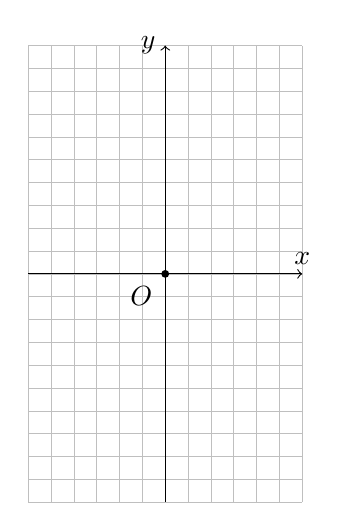
\begin{tikzpicture}[scale=0.29]
      \draw[very thin, lightgray] (-6,-10) grid (6,10) ;
      \draw[thin,->] (-6,0)--(6,0) node[above]{$x$} ;
      \draw[thin,->] (0,-10)--(0,10) node[left]{$y$} ;
      \node[fill=black,inner sep=1pt,shape=circle,label=225:$O$] %
      (O) at (0,0) {} ;
    \end{tikzpicture}
  }
  \only<2>{ %
    \centering
    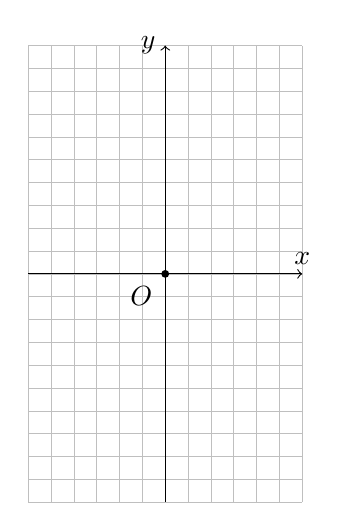
\begin{tikzpicture}[scale=0.29]
      \draw[very thin, lightgray] (-6,-10) grid (6,10) ;
      \draw[thin,->] (-6,0)--(6,0) node[above]{$x$} ;
      \draw[thin,->] (0,-10)--(0,10) node[left]{$y$} ;
      \node[fill=black,inner sep=1pt,shape=circle,label=225:$O$] %
      (O) at (0,0) {} ;
      \draw[color=red,domain=1:6] plot[id=hyp1] function{1*sqrt((x/1)**2-1)};
      \draw[color=red,domain=1:6] plot[id=hyp2] function{-1*sqrt((x/1)**2-1)};
      % EJD: these two plots are buggy, go through (0,0)
      %\draw[color=red,domain=-6:-1] plot[id=hyp3] 
      %function{1*sqrt((x/1)**2-1)};
      %\draw[color=red,domain=-6:-1] plot[id=hyp4] 
      %function{-1*sqrt((x/1)**2-1)};
      \draw[color=red,domain=1:6,rotate=180] plot[id=hyp3] 
      function{1*sqrt((x/1)**2-1)};
      \draw[color=red,domain=1:6,rotate=180] plot[id=hyp4] 
      function{-1*sqrt((x/1)**2-1)};
    \end{tikzpicture}
  }
  \only<3>{ %
    \centering
    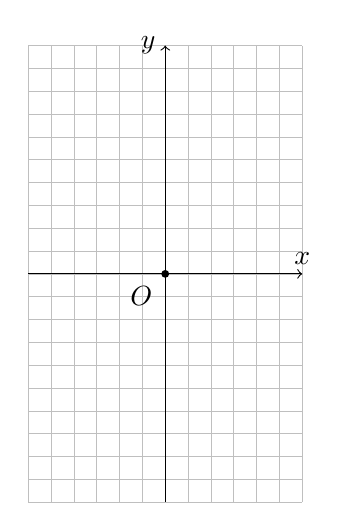
\begin{tikzpicture}[scale=0.29]
      \draw[very thin, lightgray] (-6,-10) grid (6,10) ;
      \draw[thin,->] (-6,0)--(6,0) node[above]{$x$} ;
      \draw[thin,->] (0,-10)--(0,10) node[left]{$y$} ;
      \node[fill=black,inner sep=1pt,shape=circle,label=225:$O$] %
      (O) at (0,0) {} ;
      \draw[red,domain=-6:6] plot[id=hyp5] 
      function{-1*sqrt((x/1)**2+1)};
      \draw[red,domain=-6:6] plot[id=hyp6] 
      function{1*sqrt((x/1)**2+1)};
    \end{tikzpicture}
  }
  \end{columns}
\end{frame}

\begin{frame}
  \frametitle{Intercepts of a Hyperbola}
  \begin{columns}
  \column{0.65\textwidth}
  \begin{itemize}[<+->]
  \item Unlike an ellipse in standard position, a hyperbola in
    standard position only has two intercepts.
  \item If we set $x=0$ we get $-y^2/b^2 = 1$ which is impossible
    since the LHS is negative and the RHS is positive.
  \item If we set $y=0$ we get $x^2/a^2=1$ which has two solutions,
    $x=-a$ and $x=a$.
  \item The hyperbola in standard position has two intercepts,
    $(-a,0)$ and $(a,0)$.
  \end{itemize}
  \column{0.35\textwidth}
  % EJD: graphs
  \only<1-3>{ %
    \centering
    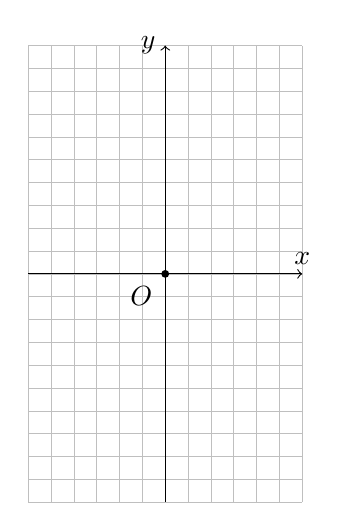
\begin{tikzpicture}[scale=0.29]
      \draw[very thin, lightgray] (-6,-10) grid (6,10) ;
      \draw[thin,->] (-6,0)--(6,0) node[above]{$x$} ;
      \draw[thin,->] (0,-10)--(0,10) node[left]{$y$} ;
      \node[fill=black,inner sep=1pt,shape=circle,label=225:$O$] %
      (O) at (0,0) {} ;
      % EJD: can I re-use plots?  Would that be a good idea?
      \draw[color=red,domain=1:6] plot[id=hyp11] function{1*sqrt((x/1)**2-1)};
      \draw[color=red,domain=1:6] plot[id=hyp12] function{-1*sqrt((x/1)**2-1)};
      \draw[color=red,domain=1:6,rotate=180] plot[id=hyp13] 
      function{1*sqrt((x/1)**2-1)};
      \draw[color=red,domain=1:6,rotate=180] plot[id=hyp14] 
      function{-1*sqrt((x/1)**2-1)};
    \end{tikzpicture}
  }
  \only<4>{ %
    \centering
    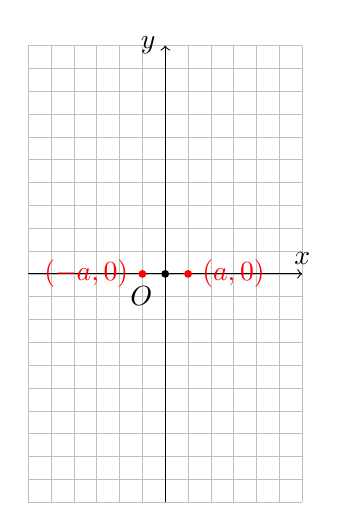
\begin{tikzpicture}[scale=0.29]
      \draw[very thin, lightgray] (-6,-10) grid (6,10) ;
      \draw[thin,->] (-6,0)--(6,0) node[above]{$x$} ;
      \draw[thin,->] (0,-10)--(0,10) node[left]{$y$} ;
      \node[fill=black,inner sep=1pt,shape=circle,label=225:$O$] %
      (O) at (0,0) {} ;
      \draw[color=red,domain=1:6] plot[id=hyp21] function{1*sqrt((x/1)**2-1)};
      \draw[color=red,domain=1:6] plot[id=hyp22] function{-1*sqrt((x/1)**2-1)};
      \draw[color=red,domain=1:6,rotate=180] plot[id=hyp23] 
      function{1*sqrt((x/1)**2-1)};
      \draw[color=red,domain=1:6,rotate=180] plot[id=hyp24] 
      function{-1*sqrt((x/1)**2-1)};
      \node[fill=red,inner sep=1pt,shape=circle,label={[red]180:$(-a,0)$}] %
      (I1) at (-1,0) {};
      \node[fill=red,inner sep=1pt,shape=circle,label={[red]0:$(a,0)$}] %
      (I2) at (1,0) {};
    \end{tikzpicture}
  }
  \end{columns}
\end{frame}

% EJD: branches? Asymptotes and Branches of a Hyperbola
\begin{frame}
  \frametitle{Asymptotes of a Hyperbola}
  \begin{columns}
  \column{0.65\textwidth}
  \begin{itemize}[<+->]
  \item Unlike an ellipse or a circle or a parabola, a hyperbola has
    two branches.
    % EJD: graphs of branches
  \item<1-> To graph a hyperbola, it helps to first draw its asymptotes.
  \item<2-> To find the asymptotes, we change the $1$ on the RHS of the
    equation to a $0$ and factor:
    \begin{equation*}
      \frac{x^2}{a^2} - \frac{y^2}{b^2} = 0
      \implies 
      \left(\frac{x}{a}+\frac{y}{b}\right)
      \left(\frac{x}{a}-\frac{y}{b}\right) = 0
    \end{equation*}
  \item<3-> That gives us two lines, $x/a + y/b = 0$ and $x/a-y/b = 0$.
  \end{itemize}
  \column{0.35\textwidth}
  \only<1-2>{ %
    \centering
    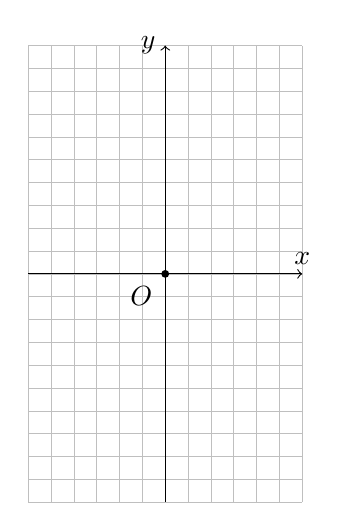
\begin{tikzpicture}[scale=0.29]
      \draw[very thin, lightgray] (-6,-10) grid (6,10) ;
      \draw[thin,->] (-6,0)--(6,0) node[above]{$x$} ;
      \draw[thin,->] (0,-10)--(0,10) node[left]{$y$} ;
      \node[fill=black,inner sep=1pt,shape=circle,label=225:$O$] %
      (O) at (0,0) {} ;
      \draw[color=red,domain=1:6] plot[id=hyp31] function{1*sqrt((x/1)**2-1)};
      \draw[color=red,domain=1:6] plot[id=hyp32] function{-1*sqrt((x/1)**2-1)};
      \draw[color=red,domain=1:6,rotate=180] plot[id=hyp33] 
      function{1*sqrt((x/1)**2-1)};
      \draw[color=red,domain=1:6,rotate=180] plot[id=hyp34] 
      function{-1*sqrt((x/1)**2-1)};
    \end{tikzpicture}
  }
  \only<3>{ %
    \centering
    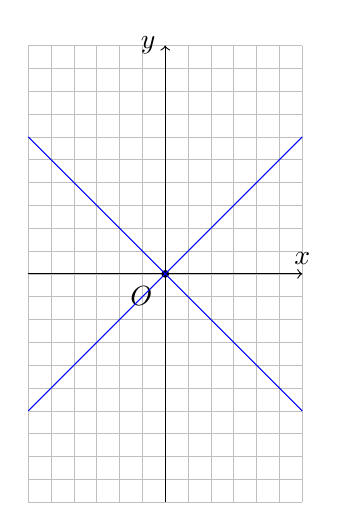
\begin{tikzpicture}[scale=0.29]
      \draw[very thin, lightgray] (-6,-10) grid (6,10) ;
      \draw[thin,->] (-6,0)--(6,0) node[above]{$x$} ;
      \draw[thin,->] (0,-10)--(0,10) node[left]{$y$} ;
      \node[fill=black,inner sep=1pt,shape=circle,label=225:$O$] %
      (O) at (0,0) {} ;
      \draw[color=red,domain=1:6] plot[id=hyp41] function{1*sqrt((x/1)**2-1)};
      \draw[color=red,domain=1:6] plot[id=hyp42] function{-1*sqrt((x/1)**2-1)};
      \draw[color=red,domain=1:6,rotate=180] plot[id=hyp43] 
      function{1*sqrt((x/1)**2-1)};
      \draw[color=red,domain=1:6,rotate=180] plot[id=hyp44] 
      function{-1*sqrt((x/1)**2-1)};
      \draw[blue] (-6,-6)--(6,6);
      \draw[blue] (-6,6)--(6,-6);
    \end{tikzpicture}
  }
  \end{columns}
\end{frame}

\begin{frame}
  \frametitle{Example: $4x^2-9y^2=36$} %EJD: change numbers
  \begin{columns}
  \column{0.65\textwidth}
  \begin{itemize}[<+->]
  \item<1-> For example, graph $4x^2-9y^2=36$
  \item<2-> Write in standard form by dividing through by $36$:
    \begin{equation*}
      \frac{x^2}{9} - \frac{y^2}{4} = 1
    \end{equation*}
  \item<3-> The intercepts are $(-3,0)$ and $(3,0)$
  \item<4-> One asymptote is $x/3+y/2=0$ or $y=-(2/3)x$
  \item<5-> The other asymptote is $y=(2/3)x$
  \item<6-> Now graph it in the ``frame'' provided by the
    asymptotes.  
  \end{itemize}
  \column{0.35\textwidth}
  \only<1-2>{ %
    \centering
    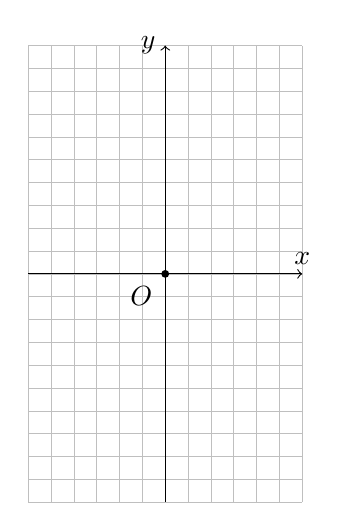
\begin{tikzpicture}[scale=0.29]
      \draw[very thin, lightgray] (-6,-10) grid (6,10) ;
      \draw[thin,->] (-6,0)--(6,0) node[above]{$x$} ;
      \draw[thin,->] (0,-10)--(0,10) node[left]{$y$} ;
      \node[fill=black,inner sep=1pt,shape=circle,label=225:$O$] %
      (O) at (0,0) {} ;
    \end{tikzpicture}
  }
  \only<3>{ %
    \centering
    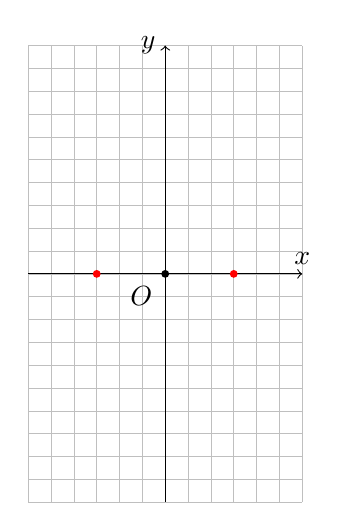
\begin{tikzpicture}[scale=0.29]
      \draw[very thin, lightgray] (-6,-10) grid (6,10) ;
      \draw[thin,->] (-6,0)--(6,0) node[above]{$x$} ;
      \draw[thin,->] (0,-10)--(0,10) node[left]{$y$} ;
      \node[fill=black,inner sep=1pt,shape=circle,label=225:$O$] %
      (O) at (0,0) {} ;
      \node[fill=red,inner sep=1pt,shape=circle] (I1) at (-3,0) {};
      \node[fill=red,inner sep=1pt,shape=circle] (I2) at (3,0) {};
    \end{tikzpicture}
  }
  \only<4>{ %
    \centering
    \begin{tikzpicture}[scale=0.29]
      \draw[very thin, lightgray] (-6,-10) grid (6,10) ;
      \draw[thin,->] (-6,0)--(6,0) node[above]{$x$} ;
      \draw[thin,->] (0,-10)--(0,10) node[left]{$y$} ;
      \node[fill=black,inner sep=1pt,shape=circle,label=225:$O$] %
      (O) at (0,0) {} ;
      \node[fill=red,inner sep=1pt,shape=circle] (I1) at (-3,0) {};
      \node[fill=red,inner sep=1pt,shape=circle] (I2) at (3,0) {};
      \draw[blue] (-6,4)--(6,-4);
    \end{tikzpicture}
  }
  \only<5>{ %
    \centering
    \begin{tikzpicture}[scale=0.29]
      \draw[very thin, lightgray] (-6,-10) grid (6,10) ;
      \draw[thin,->] (-6,0)--(6,0) node[above]{$x$} ;
      \draw[thin,->] (0,-10)--(0,10) node[left]{$y$} ;
      \node[fill=black,inner sep=1pt,shape=circle,label=225:$O$] %
      (O) at (0,0) {} ;
      \node[fill=red,inner sep=1pt,shape=circle] (I1) at (-3,0) {};
      \node[fill=red,inner sep=1pt,shape=circle] (I2) at (3,0) {};
      \draw[blue] (-6,4)--(6,-4);
      \draw[blue] (-6,-4)--(6,4);
    \end{tikzpicture}
  }
  \only<6->{ %
    \centering
    \begin{tikzpicture}[scale=0.29]
      \draw[very thin, lightgray] (-6,-10) grid (6,10) ;
      \draw[thin,->] (-6,0)--(6,0) node[above]{$x$} ;
      \draw[thin,->] (0,-10)--(0,10) node[left]{$y$} ;
      \node[fill=black,inner sep=1pt,shape=circle,label=225:$O$] %
      (O) at (0,0) {} ;
      \node[fill=red,inner sep=1pt,shape=circle] (I1) at (-3,0) {};
      \node[fill=red,inner sep=1pt,shape=circle] (I2) at (3,0) {};
      \draw[blue] (-6,4)--(6,-4);
      \draw[blue] (-6,-4)--(6,4);
      \draw[color=red,domain=3:6] plot[id=hyp51] function{2*sqrt((x/3)**2-1)};
      \draw[color=red,domain=3:6] plot[id=hyp52] function{-2*sqrt((x/3)**2-1)};
      \draw[color=red,domain=3:6,rotate=180] plot[id=hyp53] 
      function{2*sqrt((x/3)**2-1)};
      \draw[color=red,domain=3:6,rotate=180] plot[id=hyp54] 
      function{-2*sqrt((x/3)**2-1)};
    \end{tikzpicture}
  }
  \end{columns}
\end{frame}


\subsection{Shifting Conics}

\begin{frame}
  \frametitle{Shifing Parabolas}
  \begin{columns}
  \column{0.65\textwidth}
  \begin{itemize}[<+->]
  \item We start with a parabola in standard position: $y=2x^2$
  \item To shift the vertex two units to the right and one unit up, we
    \textit{subtract} $2$ from $x$ and $1$ from $y$ in the equation:
    $(y-1) = 2(x-2)^2$
  \item We can simplify the previous equation:
    $y-1 = 2(x^2-4x+4) \implies y = 2x^2-8x+9$
  \end{itemize}
  \column{0.35\textwidth}
  \only<1>{ %
    \centering
    \begin{tikzpicture}[scale=0.29]
      \draw[very thin, lightgray] (-6,-10) grid (6,10) ;
      \draw[thin,->] (-6,0)--(6,0) node[above]{$x$} ;
      \draw[thin,->] (0,-10)--(0,10) node[left]{$y$} ;
      \node[fill=black,inner sep=1pt,shape=circle,label=225:$O$] %
      (O) at (0,0) {} ;
      \draw[red] (0,0) parabola ({sqrt(5)},10);
      \draw[red] (0,0) parabola ({-sqrt(5)},10);
    \end{tikzpicture}
  }
  \only<2->{ %
    \centering
    \begin{tikzpicture}[scale=0.29]
      \draw[very thin, lightgray] (-6,-10) grid (6,10) ;
      \draw[thin,->] (-6,0)--(6,0) node[above]{$x$} ;
      \draw[thin,->] (0,-10)--(0,10) node[left]{$y$} ;
      \node[fill=black,inner sep=1pt,shape=circle,label=225:$O$] %
      (O) at (0,0) {} ;
      \clip (-6,-10)--(6,-10)--(6,10)--(-6,10)--cycle;
      \draw[red,shift={(2,1)}] (0,0) parabola ({sqrt(5)},10);
      \draw[red,shift={(2,1)}] (0,0) parabola ({-sqrt(5)},10);
    \end{tikzpicture}
  }
  \end{columns}
\end{frame}

% EJD: what about shifting down, to the left?
\begin{frame}
  \frametitle{Completing the Square}
  \begin{columns}
  \column{0.65\textwidth}
  \begin{itemize}[<+->]
  \item Conversely, given an equation like $y=2x^2-8x+9$ we can
    reverse those steps to put it in standard form.
  \item Completing the square: $y=2(x^2-4x) + 9 \implies
    y=2(x^2-4x+4-4)+9
    \implies y=2(x^2-4x+4) - 8 + 9$
  \item Finally, we have
    \begin{equation*}
      y - 1 = 2(x-2)^2
    \end{equation*}
  \item To graph it, we start with $y=2x^2$ 
  \item Then shift it $1$ unit up and $2$ units to the right.
  \end{itemize}
  \column{0.35\textwidth}
  \only<1-3>{ %
    \centering
    \begin{tikzpicture}[scale=0.29]
      \draw[very thin, lightgray] (-6,-10) grid (6,10) ;
      \draw[thin,->] (-6,0)--(6,0) node[above]{$x$} ;
      \draw[thin,->] (0,-10)--(0,10) node[left]{$y$} ;
      \node[fill=black,inner sep=1pt,shape=circle,label=225:$O$] %
      (O) at (0,0) {} ;
    \end{tikzpicture}
  }
  \only<4>{ %
    \centering
    \begin{tikzpicture}[scale=0.29]
      \draw[very thin, lightgray] (-6,-10) grid (6,10) ;
      \draw[thin,->] (-6,0)--(6,0) node[above]{$x$} ;
      \draw[thin,->] (0,-10)--(0,10) node[left]{$y$} ;
      \node[fill=black,inner sep=1pt,shape=circle,label=225:$O$] %
      (O) at (0,0) {} ;
      \draw[red] (0,0) parabola ({sqrt(5)},10);
      \draw[red] (0,0) parabola ({-sqrt(5)},10);
      %\clip (-6,-10)--(6,-10)--(6,10)--(-6,10)--cycle;
      %\draw[red,shift={(2,1)}] (0,0) parabola ({sqrt(5)},10);
      %\draw[red,shift={(2,1)}] (0,0) parabola ({-sqrt(5)},10);
    \end{tikzpicture}
  }
  \only<5->{ %
    \centering
    \begin{tikzpicture}[scale=0.29]
      \draw[very thin, lightgray] (-6,-10) grid (6,10) ;
      \draw[thin,->] (-6,0)--(6,0) node[above]{$x$} ;
      \draw[thin,->] (0,-10)--(0,10) node[left]{$y$} ;
      \node[fill=black,inner sep=1pt,shape=circle,label=225:$O$] %
      (O) at (0,0) {} ;
      \draw[red,nearly transparent] (0,0) parabola ({sqrt(5)},10);
      \draw[red,nearly transparent] (0,0) parabola ({-sqrt(5)},10);
      \clip (-6,-10)--(6,-10)--(6,10)--(-6,10)--cycle;
      \draw[red,shift={(2,1)}] (0,0) parabola ({sqrt(5)},10);
      \draw[red,shift={(2,1)}] (0,0) parabola ({-sqrt(5)},10);
    \end{tikzpicture}
  }
  \end{columns}
\end{frame}

%% \begin{frame}
%%   \frametitle{Example: $x^2-y^2-4x+3=0$}
%%   \begin{columns}
%%   \column{0.65\textwidth}
%%   \begin{itemize}[<+->]
%%   \item X
%%   \end{itemize}
%%   \column{0.35\textwidth}
%%   \end{columns}
%% \end{frame}

%% \begin{frame}
%%   \frametitle{Example: $16x^2+9y^2-36y=108$}
%%   \begin{columns}
%%   \column{0.65\textwidth}
%%   \begin{itemize}[<+->]
%%   \item X
%%   \end{itemize}
%%   \column{0.35\textwidth}
%%   \end{columns}
%% \end{frame}

\end{document}

